\chapter{Rotifera, Platyhelminthes, Molluska and
Annelida}\label{rotifera-platyhelminthes-molluska-and-annelida}

\section{Rotifers}\label{rotifers}

The \href{https://en.wikipedia.org/wiki/Rotifer}{rotifers} (Rotifera,
commonly called wheel animals) make up a phylum of microscopic and
near-microscopic pseudocoelomate animals. The word ``rotifer'' is
derived from a Latin word meaning ``wheel-bearer'', due to the corona
around the mouth that in concerted sequential motion resembles a wheel
(though the organ does not actually rotate). They were first described
by Rev.~John Harris in 1696, and other forms were described by \href{https://en.wikipedia.org/wiki/Antonie_van_Leeuwenhoek}{Antonie
van Leeuwenhoek} in 1703. Most rotifers are around 0.1--0.5 mm long
(although their size can range from 50 μm to over 2 mm), and are common
in freshwater environments throughout the world with a few saltwater
species; for example, those of genus Synchaeta. Some rotifers are free
swimming and truly planktonic, others move by inchworming along a
substrate, and some are sessile, living inside tubes or gelatinous
holdfasts that are attached to a substrate. About 25 species are
colonial (e.g., Sinantherina semibullata), either sessile or planktonic.
Rotifers are an important part of the freshwater zooplankton, being a
major foodsource and with many species also contributing to the
decomposition of soil organic matter.

Rotifers have bilateral symmetry and a variety of different shapes. The
body of a rotifer is divided into a head, trunk, and foot, and is
typically somewhat cylindrical. There is a well-developed cuticle, which
may be thick and rigid, giving the animal a box-like shape, or flexible,
giving the animal a worm-like shape; such rotifers are respectively
called loricate and illoricate. Rigid cuticles are often composed of
multiple plates, and may bear spines, ridges, or other ornamentation.
Their cuticle is non-chitinous and is formed from sclerotized proteins.

The most distinctive feature of rotifers is the presence of a ciliated
structure, called the corona, on the head. In the more primitive
species, this forms a simple ring of cilia around the mouth from which
an additional band of cilia stretches over the back of the head. In the
great majority of rotifers, however, this has evolved into a more
complex structure. The trunk forms the major part of the body, and
encloses most of the internal organs. The foot projects from the rear of
the trunk, and is usually much narrower, giving the appearance of a
tail. The cuticle over the foot often forms rings, making it appear
segmented, although the internal structure is uniform. Many rotifers can
retract the foot partially or wholly into the trunk. The foot ends in
from one to four toes, which, in sessile and crawling species, contain
adhesive glands to attach the animal to the substratum. In many
free-swimming species, the foot as a whole is reduced in size, and may
even be absent.

Rotifers are dioecious and reproduce sexually or parthenogenetically.
They are sexually dimorphic, with the females always being larger than
the males. In some species, this is relatively mild, but in others the
female may be up to ten times the size of the male. In parthenogenetic
species, males may be present only at certain times of the year, or
absent altogether. The female reproductive system consists of one or two
ovaries, each with a vitellarium gland that supplies the eggs with yolk.
Together, each ovary and vitellarium form a single syncitial structure
in the anterior part of the animal, opening through an oviduct into the
cloaca. Males do not usually have a functional digestive system, and are
therefore short-lived, often being sexually fertile at birth. They have
a single testicle and sperm duct, associated with a pair of glandular
structures referred to as prostates (unrelated to the vertebrate
prostate). The sperm duct opens into a gonopore at the posterior end of
the animal, which is usually modified to form a penis. The gonopore is
homologous to the cloaca of females, but in most species has no
connection to the vestigial digestive system, which lacks an anus.
Fertilization is internal. The male either inserts his penis into the
female's cloaca or uses it to penetrate her skin, injecting the sperm
into the body cavity. The egg secretes a shell, and is attached either
to the substratum, nearby plants, or the female's own body. A few
species, such as Rotaria, are ovoviviparous, retaining the eggs inside
their body until they hatch. Most species hatch as miniature versions of
the adult. Sessile species, however, are born as free-swimming larvae,
which closely resemble the adults of related free-swimming species.
Females grow rapidly, reaching their adult size within a few days, while
males typically do not grow in size at all.

\section{Platyhelminthes}\label{platyhelminthes}

The \href{https://en.wikipedia.org/wiki/Flatworm}{flatworms}, flat
worms, Platyhelminthes, Plathelminthes, or platyhelminths (from the
Greek platy, meaning ``flat'' and helminth-, meaning ``worm'') are a
phylum of relatively simple bilaterian, unsegmented, soft-bodied
invertebrates. Unlike other bilaterians, they are acoelomates (having no
body cavity), and have no specialized circulatory and respiratory
organs, which restricts them to having flattened shapes that allow
oxygen and nutrients to pass through their bodies by diffusion. The
digestive cavity has only one opening for both ingestion (intake of
nutrients) and egestion (removal of undigested wastes); as a result, the
food cannot be processed continuously.

Free-living flatworms are mostly predators, and live in water or in
shaded, humid terrestrial environments, such as leaf litter. Cestodes
(tapeworms) and trematodes (flukes) have complex life-cycles, with
mature stages that live as parasites in the digestive systems of fish or
land vertebrates, and intermediate stages that infest secondary hosts.
The eggs of trematodes are excreted from their main hosts, whereas adult
cestodes generate vast numbers of hermaphroditic, segment-like
proglottids that detach when mature, are excreted, and then release
eggs. Unlike the other parasitic groups, the monogeneans are external
parasites infesting aquatic animals, and their larvae metamorphose into
the adult form after attaching to a suitable host.

Over half of all known flatworm species are parasitic, and some do
enormous harm to humans and their livestock. Schistosomiasis, caused by
one genus of trematodes, is the second-most devastating of all human
diseases caused by parasites, surpassed only by malaria.
Neurocysticercosis, which arises when larvae of the pork tapeworm \emph{Taenia
solium} penetrate the central nervous system, is the major cause of
acquired epilepsy worldwide. The threat of flatworm parasites to humans
in developed countries is rising because of the popularity of raw or
lightly cooked foods, and imports of food from high-risk areas. In less
developed countries, people often cannot afford the fuel required to
cook food thoroughly, and poorly designed water-supply and irrigation
projects increase the dangers presented by poor sanitation and
unhygienic farming.

In traditional medicinal texts, Platyhelminthes are divided into

\begin{itemize}
\tightlist
\item
  Turbellaria
\item
  Cestoda
\item
  Trematoda
\item
  Monogenea
\end{itemize}

\section{Turbellaria}\label{turbellaria}

\href{https://en.wikipedia.org/wiki/Turbellaria}{Turbellaria} have about
4,500 species, are mostly free-living, and range from 1 mm (0.039 in) to
600 mm in length. Most are predators or scavengers, and terrestrial
species are mostly nocturnal and live in shaded, humid locations, such
as leaf litter or rotting wood. However, some are symbiotes of other
animals, such as crustaceans, and some are parasites. Free-living
turbellarians are mostly black, brown or gray, but some larger ones are
brightly colored.

\section{\texorpdfstring{\emph{Dugesia}}{Dugesia}}\label{dugesia}

\href{https://en.wikipedia.org/wiki/Dugesia}{\emph{Dugesia}} is a
representatives of the class Turbellaria. These common flatworms are
found in freshwater habitats of Africa, Europe, Middle East, Asia and
Australia. \emph{Dugesia} species have an elongated body with a slightly
triangle-shaped head. Usually they have grey, brown or black colors on
the dorsal body surface, the ventral surface uses to be paler. These
animals have a couple of eyes constituted by a multicellular pigmented
cup with many retinal cells to detect the amount of light in the nearby
environment. Sometimes they present supernumerary eyes. At the anterior
part of the body, behind the eyes level, they have two of structures
called auricles that give the triangle look to the `head' and that allow
them to detect the intensity of water current. These auricles are free
of pigment and rhabdites. Each side of the anterior margin of the head
have between 5 and 10 shallow sensory fossae, their number depends on
the species or the individual. The sensory fossae and the auricle
grooves are supplied with many nerve endings.

\emph{Dugesia} digestion tract consists of a central non-pigmented
tubular pharynx. Like the other triclads \emph{Dugesia} gut consists in
three ramified branches. Each branch consists of ceca, which delivers
the nutrients to the body. This worm has a sac digestive plan, that is,
it does not have a separate opening for waste excretion.

In \emph{Dugesia} the ovaries are ventrally situated, they start just
behind the brain, usually at the level of the fourth intestinal branch.
The bursal canal runs on the right side of the copulatory apparatus and
above the atrium.

They are hermaphrodites. Many species can reproduce both sexually and
asexually (by parthenogenesis or by fission).

\section{\texorpdfstring{View Prepared Slides of
\emph{Dugesia}}{View Prepared Slides of Dugesia}}\label{view-prepared-slides-of-dugesia}

\begin{enumerate}
\def\labelenumi{\arabic{enumi}.}
\tightlist
\item
  \emph{Dugesia} w.m. (Figure \ref{fig:dugesia})

  \begin{itemize}
  \tightlist
  \item
    Identify: highly branched gastrovascular cavity (GVC), pharynx,
    pharyngeal pouch, eyespots, auricles. Be sure to differentiate
    between anterior and posterior ends.
  \end{itemize}
\item
  \emph{Dugesia} x.s. 3 regions (Figure \ref{fig:dugesiaxs})

  \begin{itemize}
  \tightlist
  \item
    Identify: Anterior region: gastrovascular cavity (GVC) surrounded by
    endoderm; pharynx region: pharynx, GVC surrounded by endoderm,
    epidermis, testis, dorsoventral muscles; posterior end: epidermis,
    GVC surrounded by endoderm, dorsoventral muscles, ventral nerve cord
  \end{itemize}
\end{enumerate}

\begin{figure}

{\centering 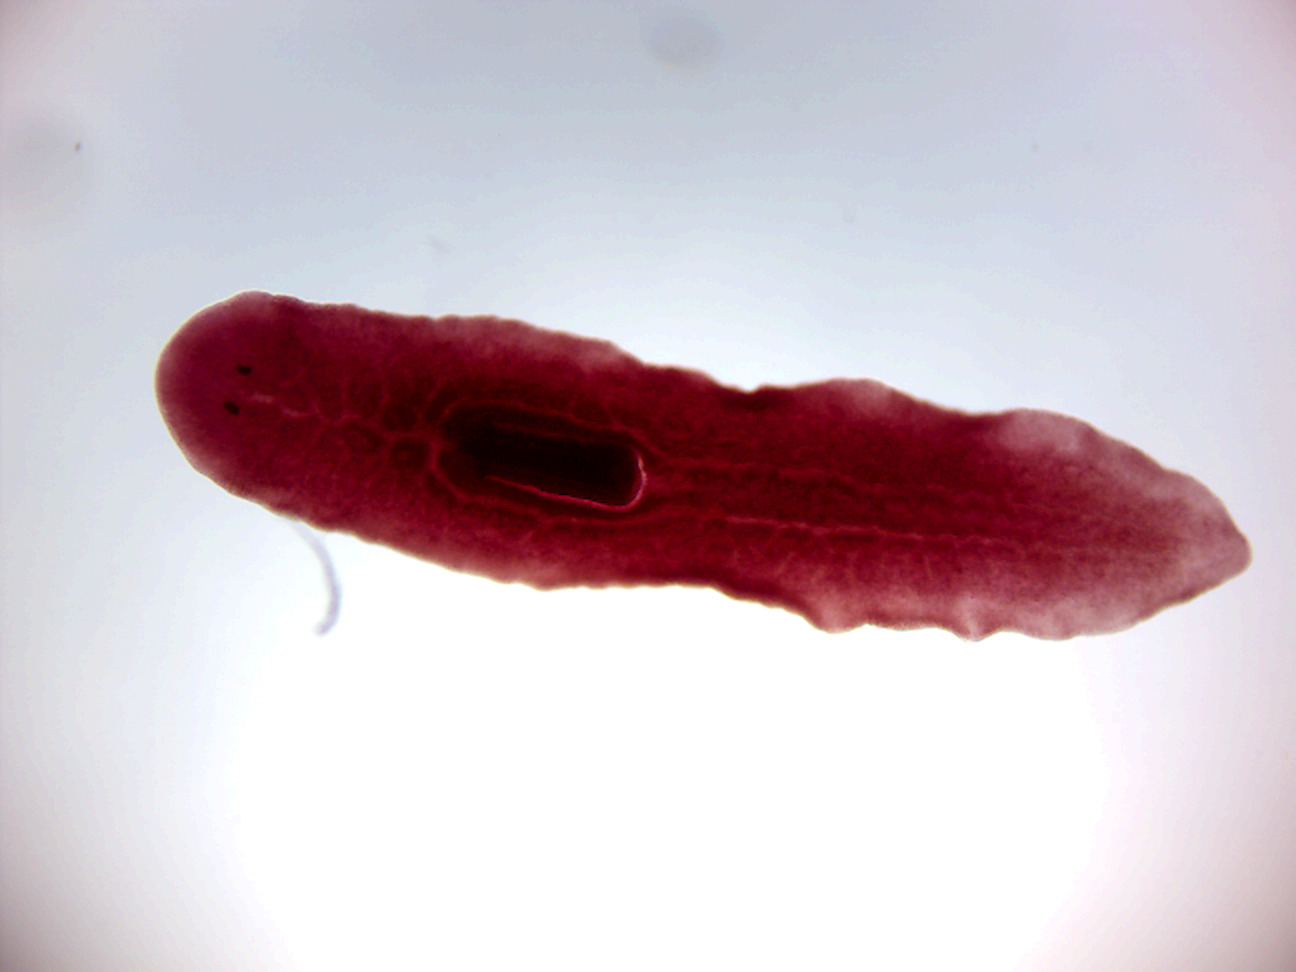
\includegraphics[width=0.7\linewidth]{./figures/rotifera/dugesia}

}

\caption{\emph{Dugesia}.}\label{fig:dugesia}
\end{figure}

\begin{figure}

{\centering 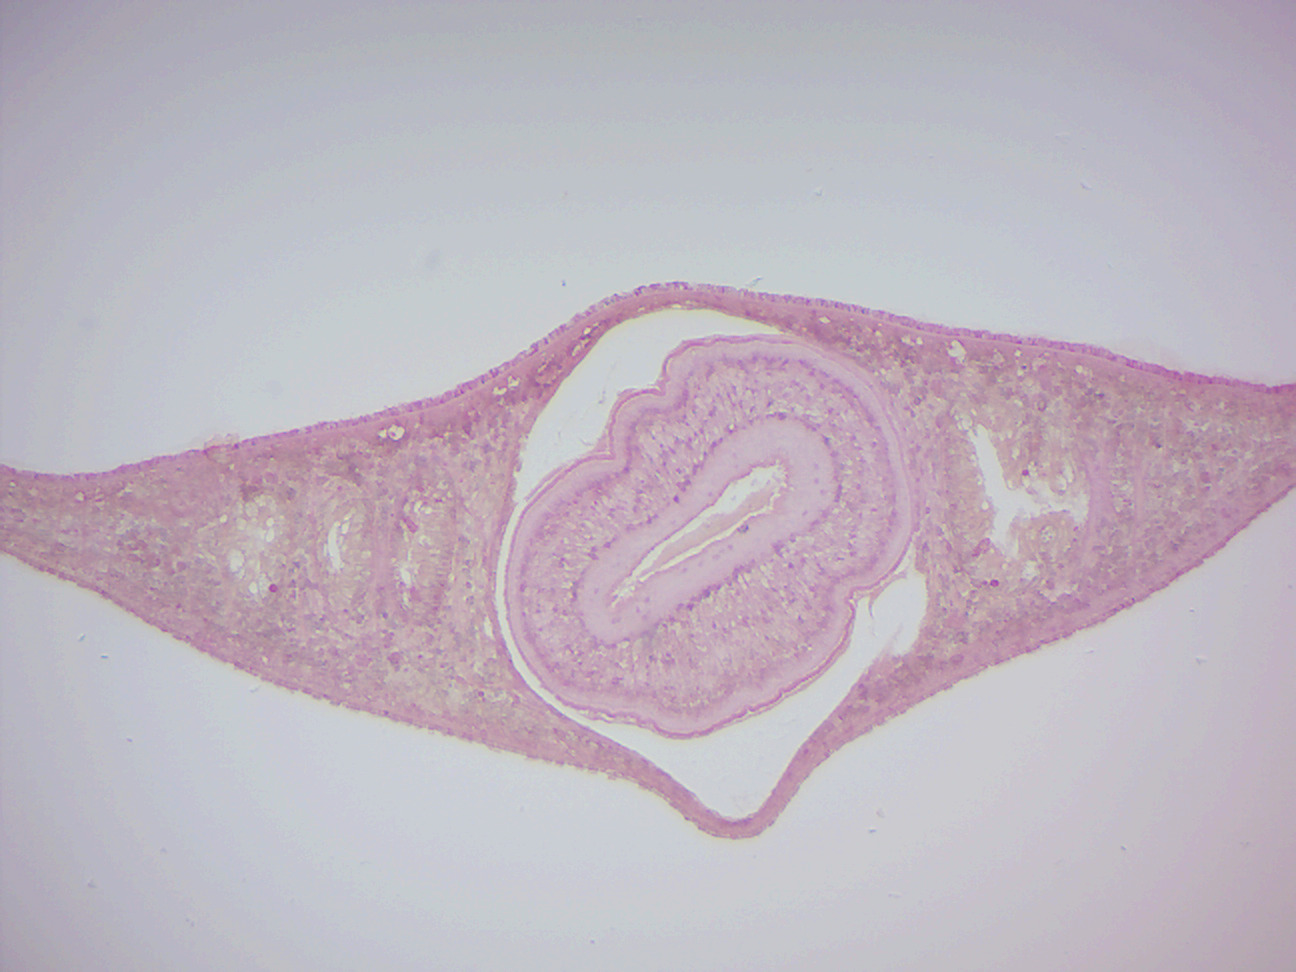
\includegraphics[width=0.7\linewidth]{./figures/rotifera/dugesia_xs}

}

\caption{\emph{Dugesia} cross section through pharynx region.}\label{fig:dugesiaxs}
\end{figure}

\section{Cestoda}\label{cestoda}

\href{https://en.wikipedia.org/wiki/Cestoda}{\emph{Cestoda}} are
commonly called tapeworms. All cestodes are parasitic and their life
histories vary, but typically they live in the digestive tracts of
vertebrates as adults, and often in the bodies of other species of
animals as juveniles. Over a thousand species have been described, and
all vertebrate species may be parasitized by at least one species of
tapeworm.

Humans are subject to infection by several species of tapeworms if they
eat undercooked meat such as pork
(\href{https://en.wikipedia.org/wiki/Taenia_solium}{\emph{Taenia
solium}}), beef
(\href{https://en.wikipedia.org/wiki/Taenia_saginata}{\emph{T.
saginata}}), and fish (\emph{Diphyllobothrium} spp.), or if they live
in, or eat food prepared in, conditions of poor hygiene
(\emph{Hymenolepis} or \emph{Echinococcus} species).

\emph{T. saginata}, the beef tapeworm, can grow up to 20 m. Species
using small vertebrates as hosts, though, tend to be small.

Tapeworm parasites of vertebrates have a long history: recognizable
clusters of cestode eggs, one with a developing larva, have been
discovered in fossil feces (coprolites) of a shark dating to the mid- to
late Permian, some 270 million years ago.

The worm's head, known as a scolex, attaches to the intestine of the
definitive host. In some species, the scolex is dominated by bothria, or
``sucking grooves'' that function like suction cups. Other species have
hooks and suckers that aid in attachment.

The main nerve centre of a cestode is a cerebral ganglion in its scolex.
Motor and sensory innervation depends on the number of nerves in and
complexity of the scolex. Smaller nerves emanate from the ganglion to
supply the general body muscular and sensory ending. The cirrus and
vagina are innervated, and sensory endings around the genital pore are
more plentiful than other areas. Sensory function includes both
tactoreception (touch) and chemoreception (smell or taste). Some nerves
are only temporary.

The body is composed of successive segments called proglottids. The sum
of the proglottids is called a strobila, which is thin, and resembles a
strip of tape. From this is derived the common name ``tapeworm''.
Proglottids are continually produced by the neck region of the scolex,
as long as the scolex is attached and alive. Like some other flatworms,
cestodes use flame cells (protonephridia), located in the proglottids,
for excretion. Mature proglottids are released from the tapeworm's end
segment and leave the host in feces or migrate as independent motile
proglottids. The proglottids farthest away from the scolex are the
mature ones containing eggs. Mature proglottids are essentially bags of
eggs, each of which is infective to the proper intermediate host.

Once anchored to the host's intestinal wall, the tapeworm absorbs
nutrients through its skin as the food being digested by the host flows
over and around it. Soon, it begins to grow a tail composed of a series
of segments, with each segment containing an independent digestive
system and reproductive tract. Older segments are pushed toward the tip
of the tail as new segments are produced by the neckpiece. By the time a
segment has reached the end of the worm's tail, only the reproductive
tract is left. The segment then separates, carrying the tapeworm eggs
out of the definitive host as what is basically a sack of eggs.

True tapeworms are exclusively hermaphrodites, with both male and female
reproductive systems in their bodies. The reproductive system includes
one or more testes, cirri, vas deferens, and seminal vesicles as male
organs, and a single lobed or unlobed ovary with the connecting oviduct
and uterus as female organs. The common external opening for both male
and female reproductive systems is known as the genital pore, which is
situated at the surface opening of the cup-shaped atrium. Though they
are sexually hermaphroditic, self-fertilization is a rare phenomenon. To
permit hybridization, cross-fertilization between two individuals is
often practiced for reproduction. During copulation, the cirri of one
individual connect with those of the other through the genital pore, and
then spermatozoa are exchanged.

The lifecycle of tapeworms is simple in the sense that no asexual phases
occur as in other flatworms, but complicated in that at least one
intermediate host is required as well as the definitive host. Many
tapeworms have a two-phase lifecycle with two types of hosts. The adult
\emph{Taenia saginata} lives in the gut of a primate such as a human, but more
alarming is \emph{Taenia solium}, which can form cysts in the human brain.
Proglottids leave the body through the anus and fall onto the ground,
where they may be eaten with grass by an animal such as a cow. If the
tapeworm is compatible with the eating animal, this animal becomes an
intermediate host. The juvenile form of the worm enters through the
mouth, but then migrates and establishes as a cyst in the intermediate
host's body tissues such as muscles, rather than the gut. This can cause
more damage to the intermediate host than it does to its definitive
host. The parasite completes its lifecycle when the intermediate host
passes on the parasite to the definitive host. This is usually done by
the definitive host eating a suitably infected intermediate host, e.g.,
a human eating raw or undercooked meat.

\section{\texorpdfstring{View Prepared Slides of
\emph{Taenia}}{View Prepared Slides of Taenia}}\label{view-prepared-slides-of-taenia}

\begin{enumerate}
\def\labelenumi{\arabic{enumi}.}
\tightlist
\item
  \href{https://en.wikipedia.org/wiki/Taenia_pisiformis}{\emph{Taenia
  pisoformis}}. Identify

  \begin{itemize}
  \tightlist
  \item
    Scolex: rostellum with hooks, suckers (Figure \ref{fig:scolex})
  \item
    Mature proglottid: testes, sperm duct, excretory duct, uterus,
    vagina, ovary, genital pore, yolk gland (Figure
    \ref{fig:proglottid})
  \item
    Gravid proglottid: zygotes in branched uterus (Figure
    \ref{fig:gravid})
  \end{itemize}
\item
  \emph{Taenia solium} cysticercus w.m. (Figure \ref{fig:cysticercus}).

  \begin{itemize}
  \tightlist
  \item
    Identify: scolex, neck, bladder
  \end{itemize}
\end{enumerate}

\begin{figure}

{\centering 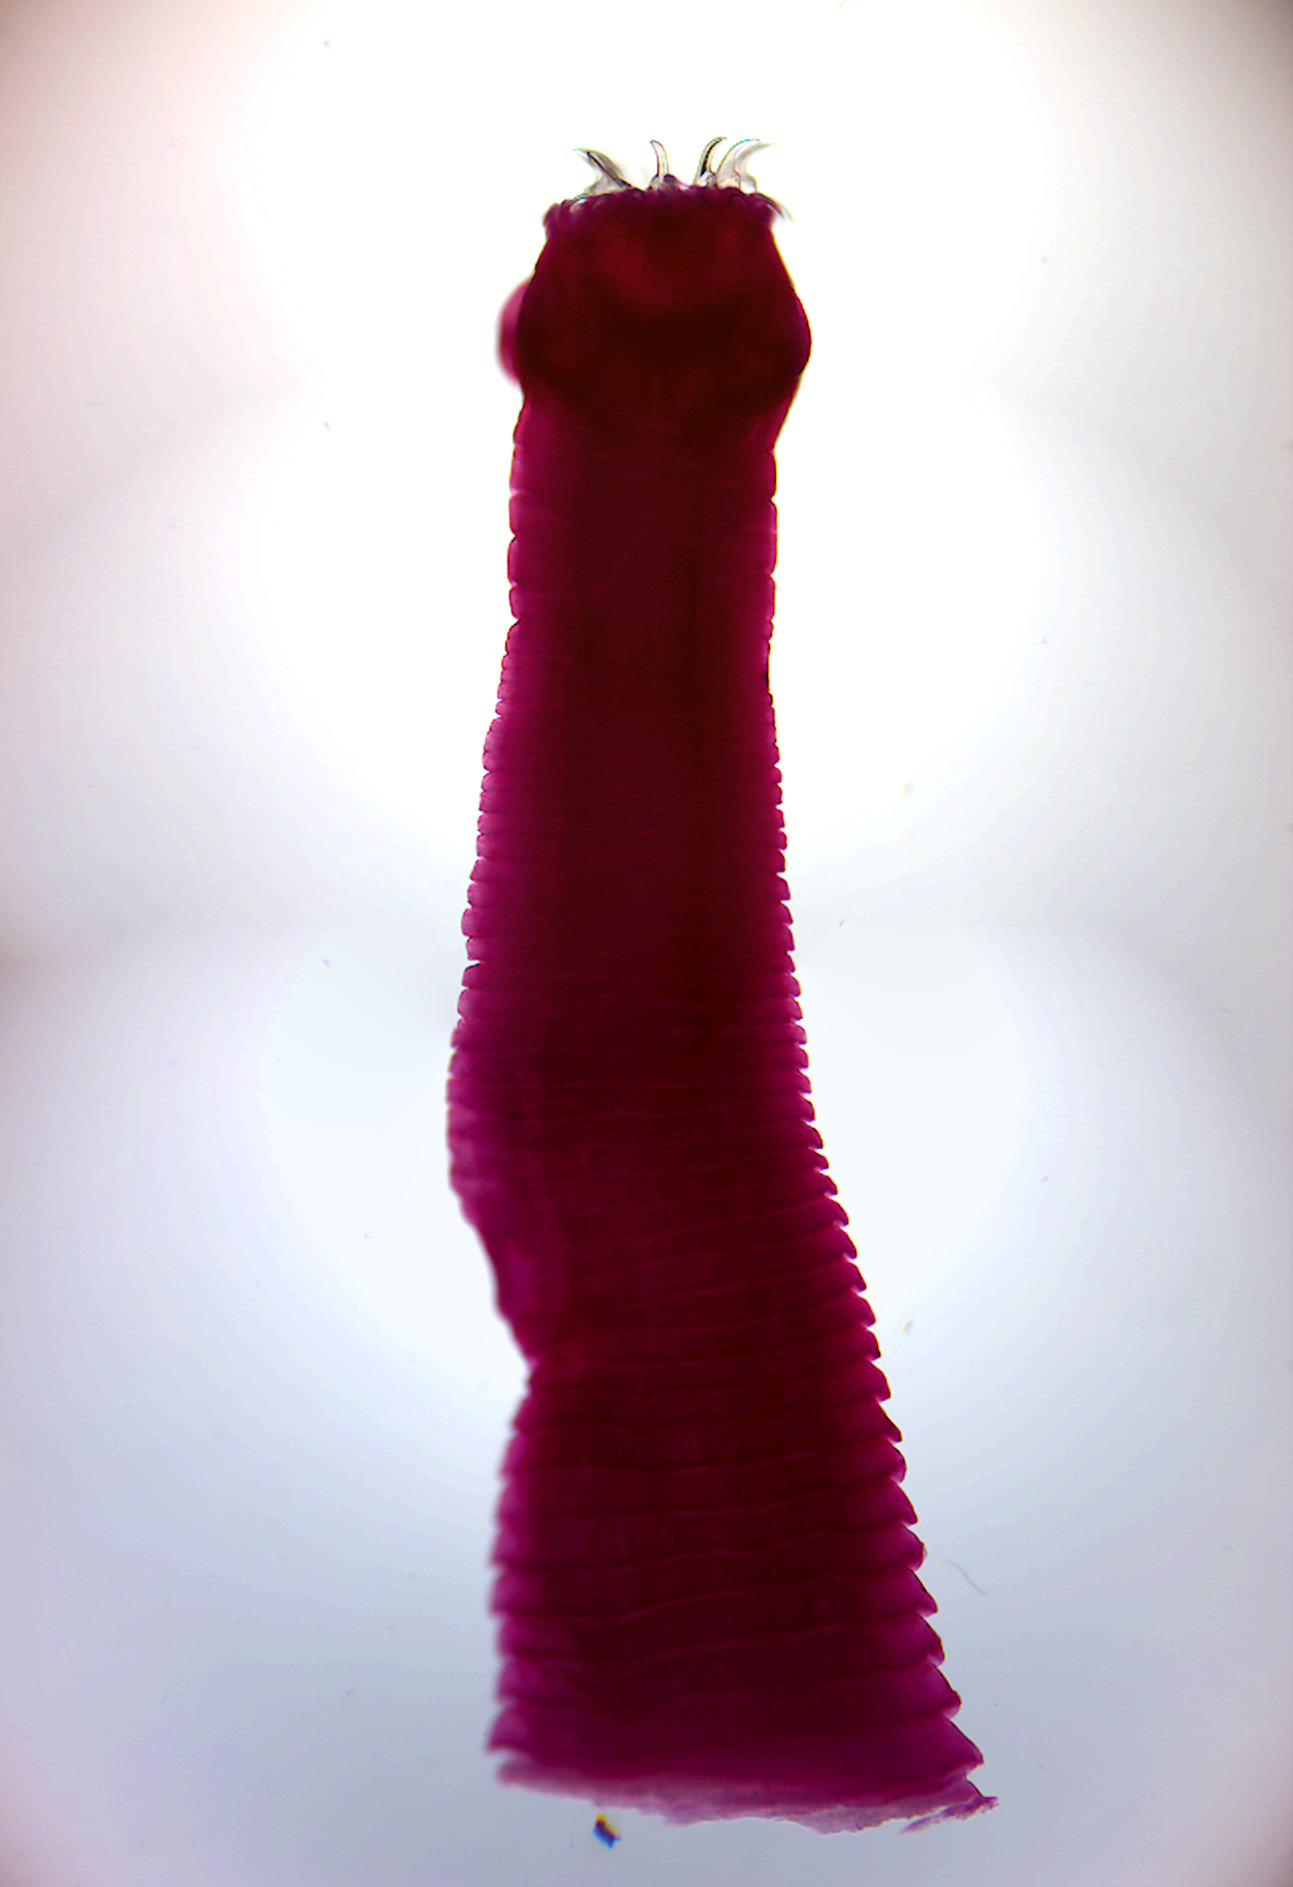
\includegraphics[width=0.7\linewidth]{./figures/rotifera/taenia_scolex}

}

\caption{\emph{Taenia} scolex.}\label{fig:scolex}
\end{figure}

\begin{figure}

{\centering 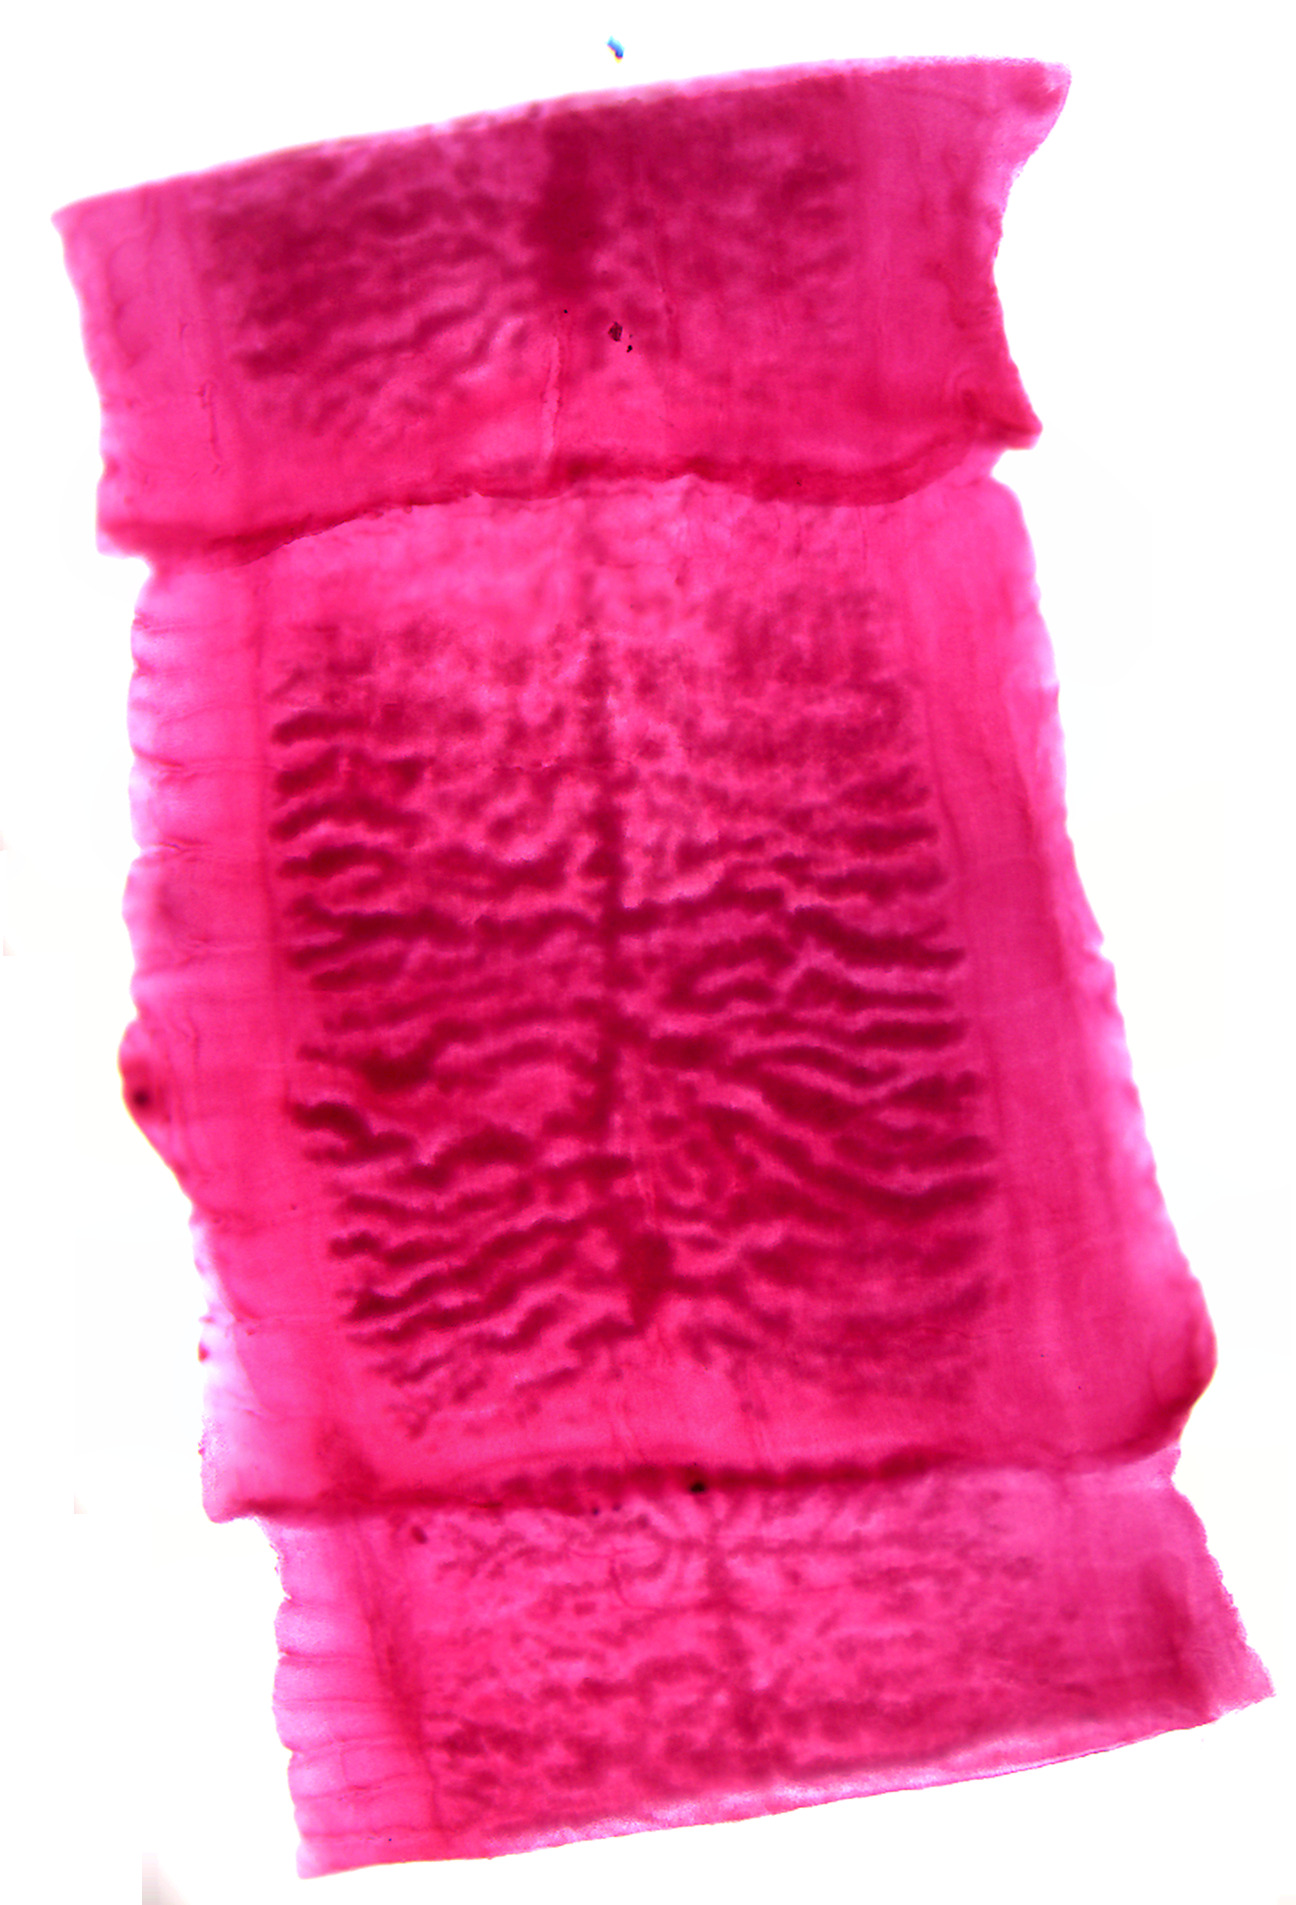
\includegraphics[width=0.7\linewidth]{./figures/rotifera/taenia_proglottids}

}

\caption{\emph{Taenia} proglottid.}\label{fig:proglottid}
\end{figure}

\begin{figure}

{\centering 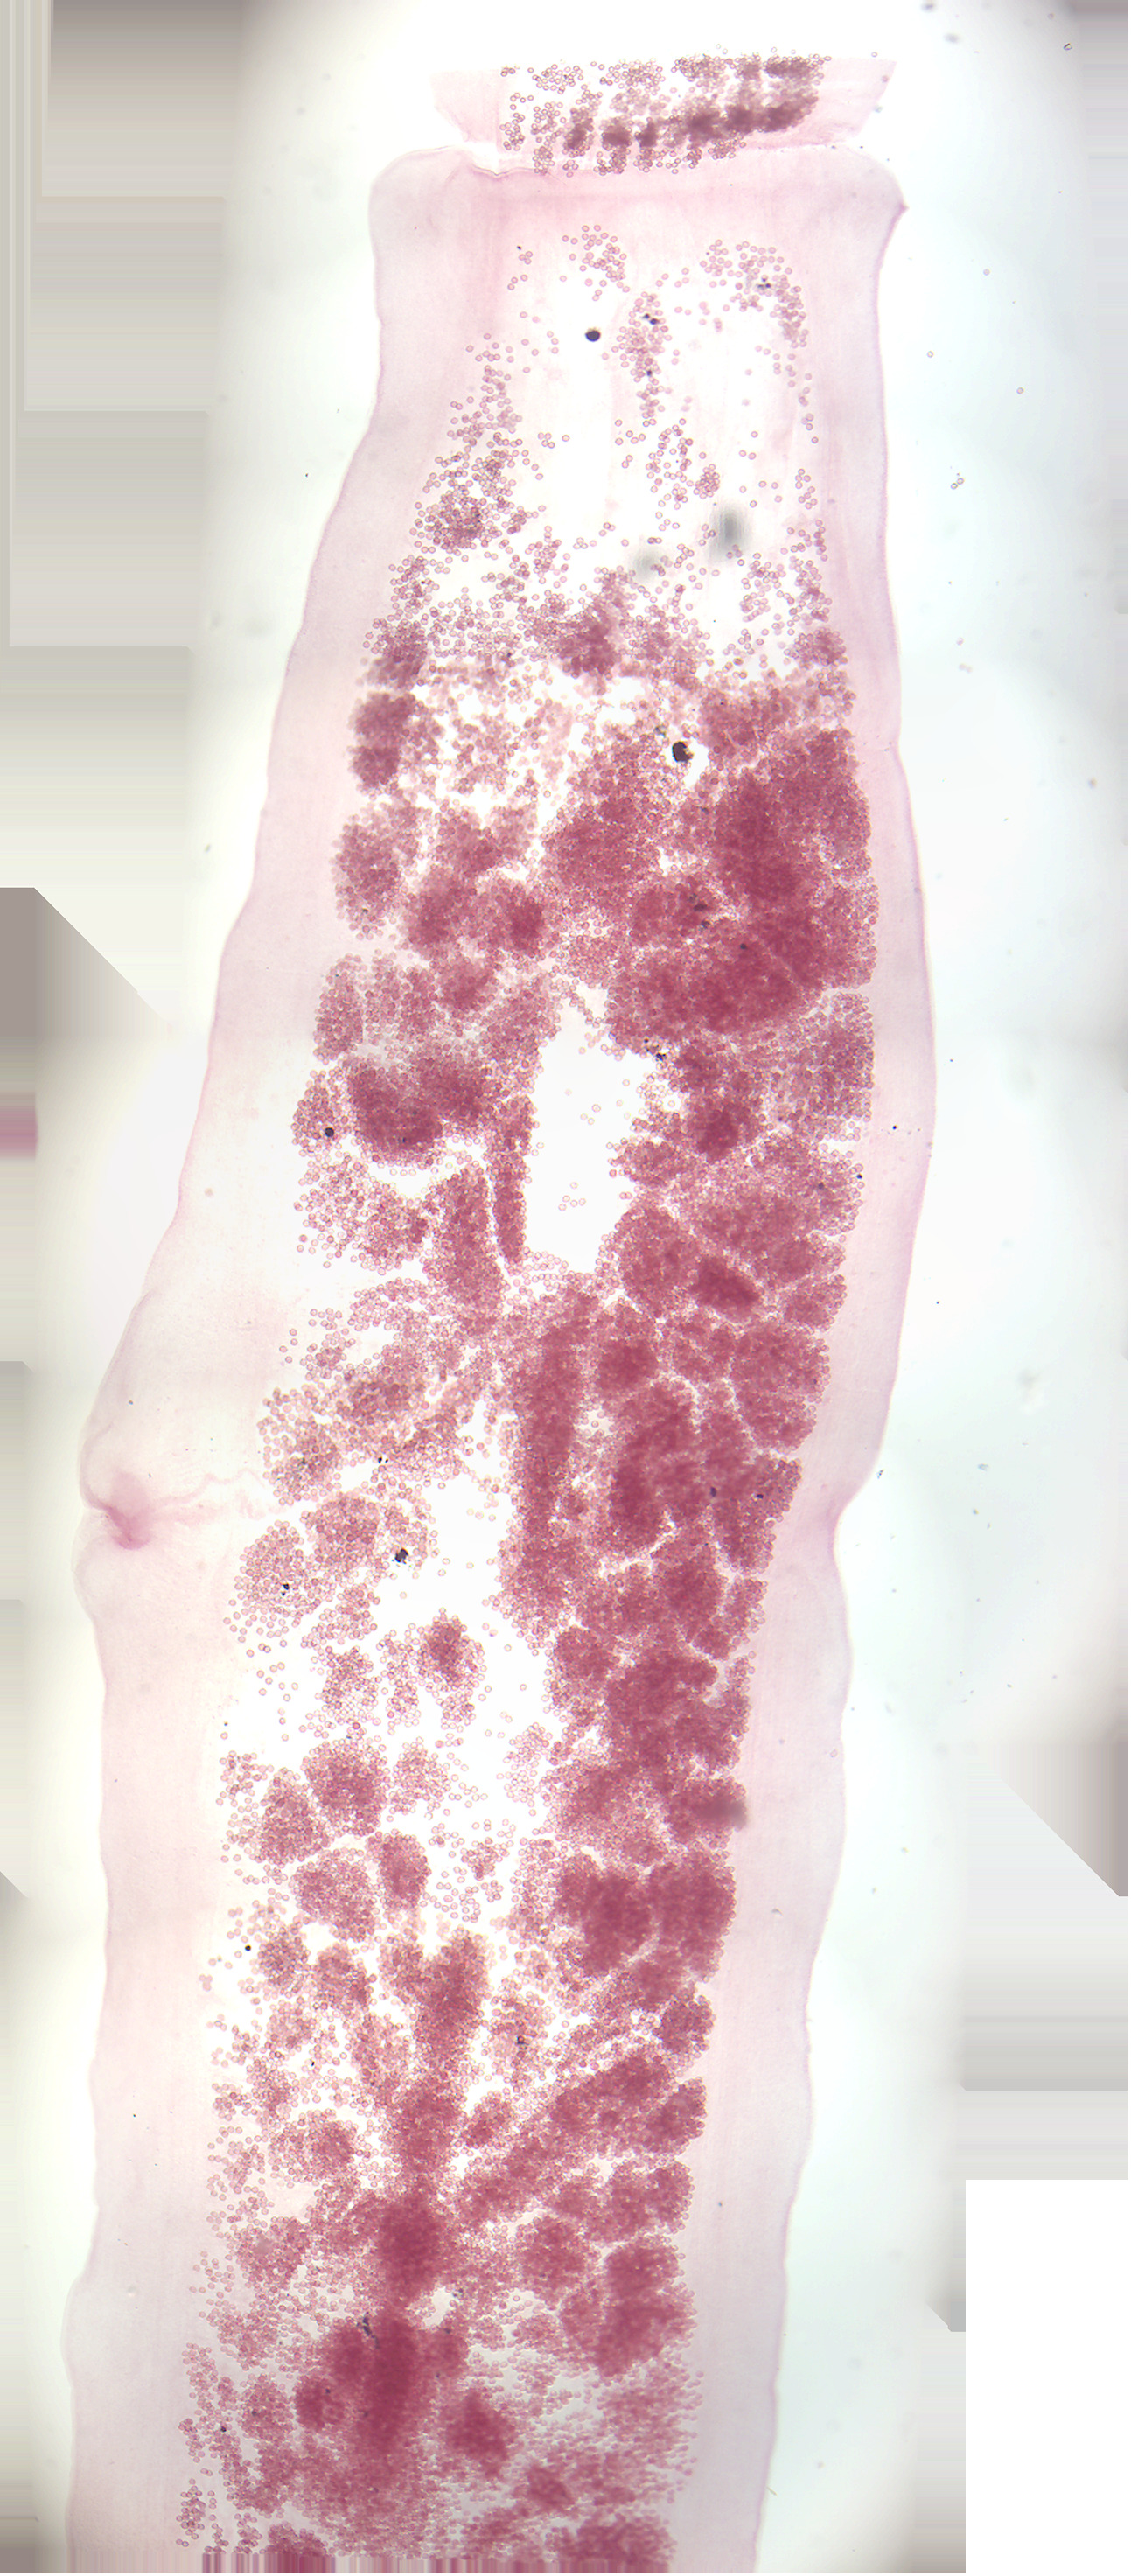
\includegraphics[width=0.7\linewidth]{./figures/rotifera/taenia_gravid_proglottid}

}

\caption{\emph{Taenia} gravid proglottid.}\label{fig:gravid}
\end{figure}

\begin{figure}

{\centering 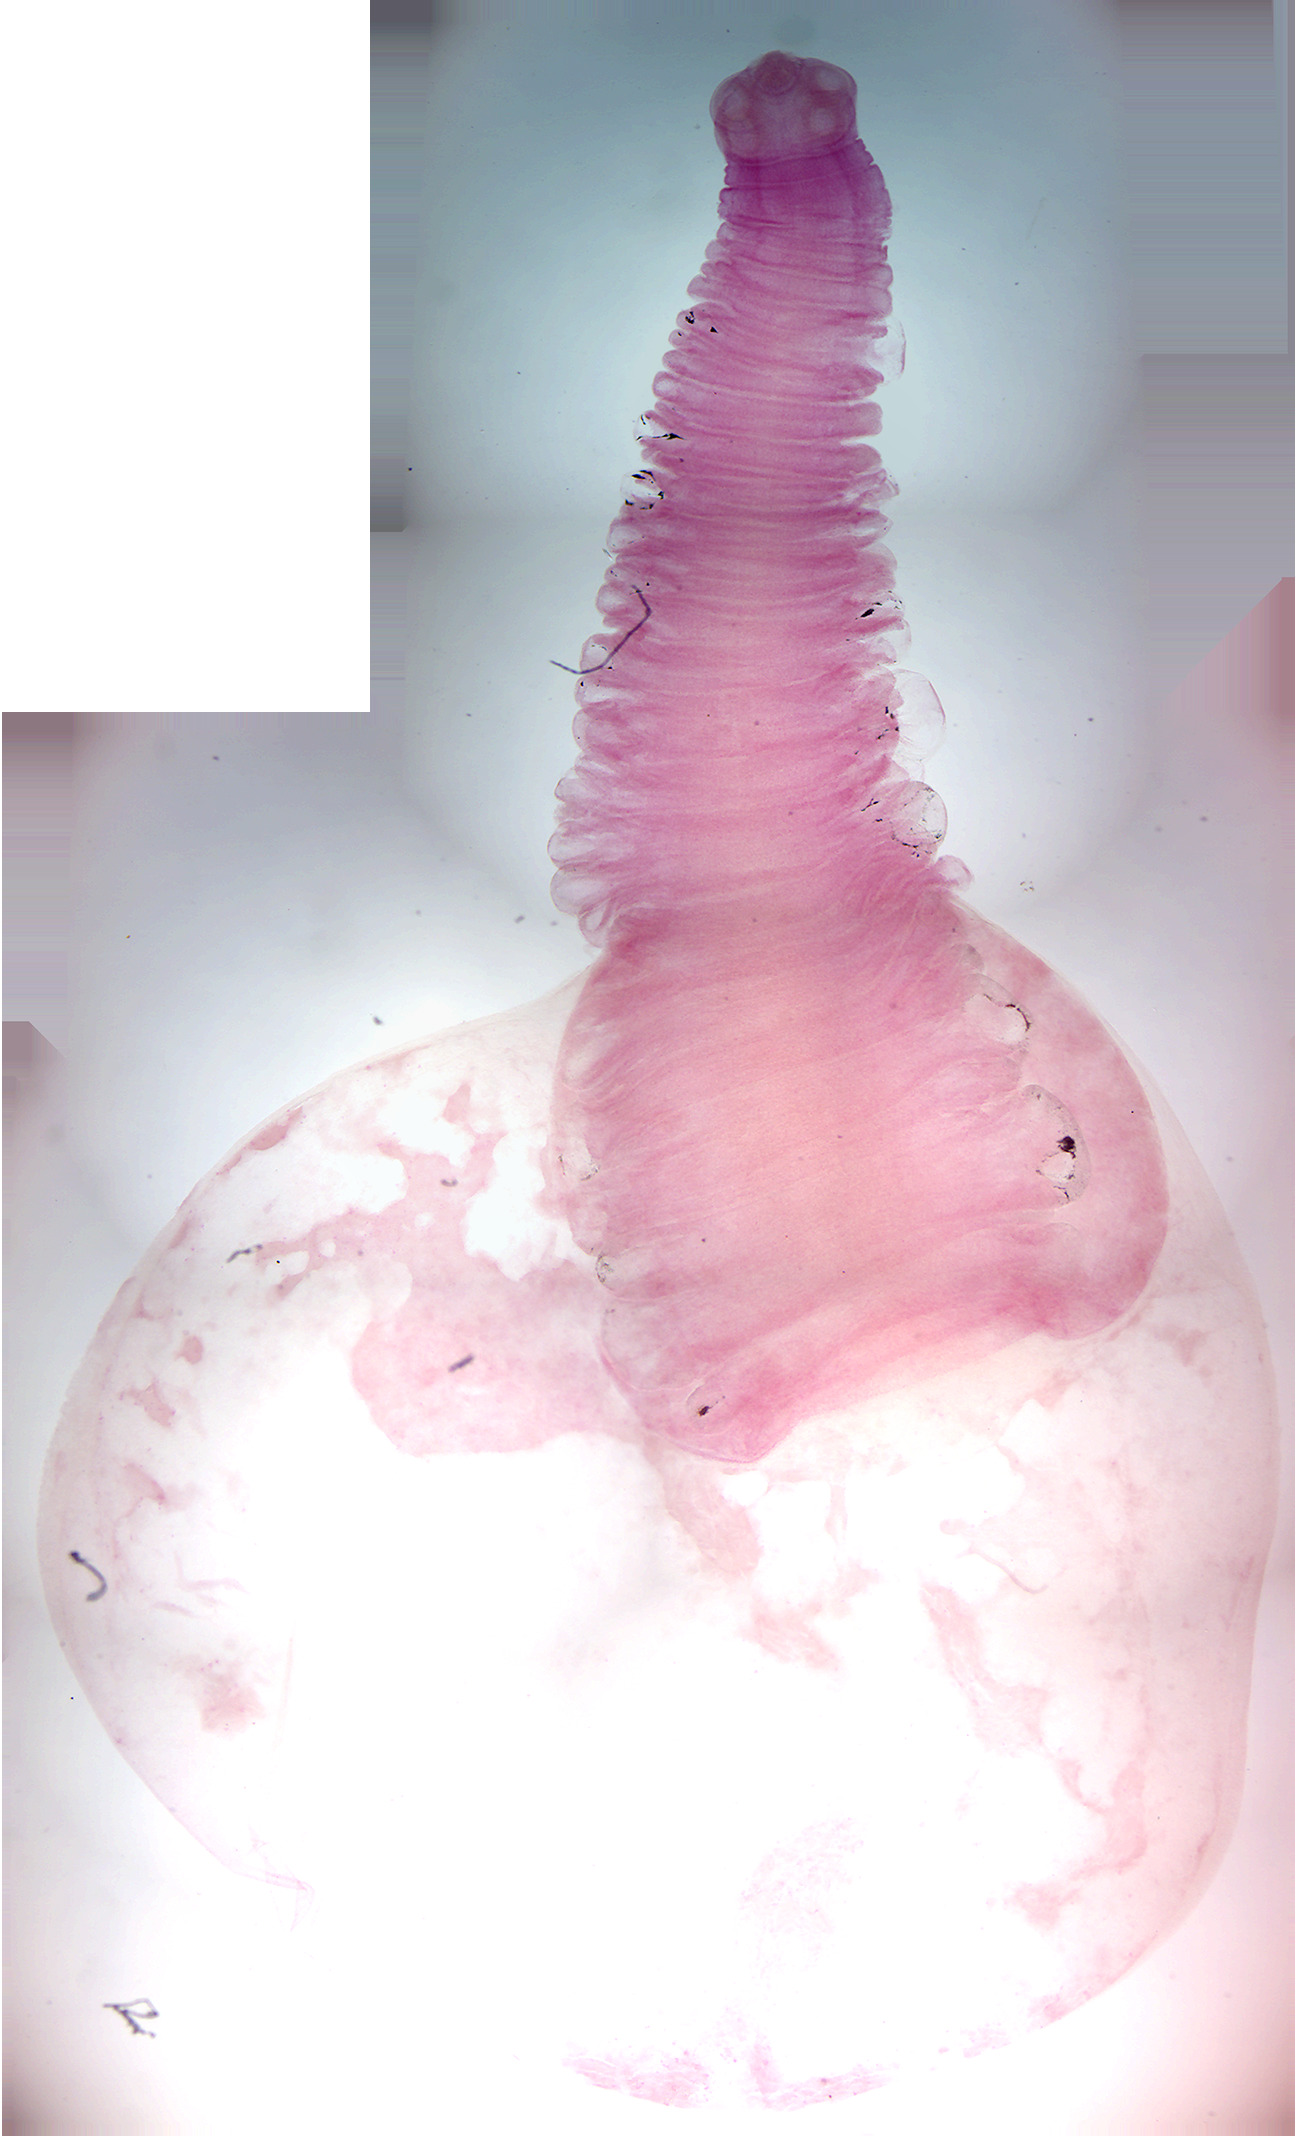
\includegraphics[width=0.7\linewidth]{./figures/rotifera/taenia_solium_cysticercus}

}

\caption{\emph{Taenia solium} cysticercus.}\label{fig:cysticercus}
\end{figure}

\section{Trematoda}\label{trematoda}

The \href{https://en.wikipedia.org/wiki/Trematoda}{trematodes} or flukes
include 18,000 to 24,000 species, divided into two subclasses. Nearly
all trematodes are parasites of mollusks and vertebrates. Most
trematodes have a complex life cycle with at least two hosts. The
primary host, where the flukes sexually reproduce, is a vertebrate. The
intermediate host, in which asexual reproduction occurs, is usually a
snail.

Trematodes are flattened oval or worm-like animals, usually no more than
a few centimeters in length, although species as small as 1 millimeter)
are known. Their most distinctive external feature is the presence of
two suckers, one close to the mouth, and the other on the underside of
the animal.

The body surface of trematodes comprises a tough syncitial tegument,
which helps protect against digestive enzymes in those species that
inhabit the gut of larger animals. It is also the surface of gas
exchange; there are no respiratory organs. The mouth is located at the
forward end of the animal, and opens into a muscular, pumping pharynx.
The pharynx connects, via a short oesophagus, to one or two blind-ending
caeca, which occupy most of the length of the body. In some species, the
caeca are themselves branched. As in other flatworms, there is no anus,
and waste material must be egested through the mouth.

Although the excretion of nitrogenous waste occurs mostly through the
tegument, trematodes do possess an excretory system, which is instead
mainly concerned with osmoregulation. This consists of two or more
protonephridia, with those on each side of the body opening into a
collecting duct. The two collecting ducts typically meet up at a single
bladder, opening to the exterior through one or two pores near the
posterior end of the animal.

The brain consists of a pair of ganglia in the head region, from which
two or three pairs of nerve cords run down the length of the body.
Trematodes generally lack any specialized sense organs, although some
ectoparasitic species do possess one or two pairs of simple ocelli.

Most trematodes are simultaneous hermaphrodites, having both male and
female organs. There are usually two testes, with sperm ducts that join
together on the underside of the front half of the animal. This final
part of the male system varies considerably in structure between
species, but may include sperm storage sacs and accessory glands, in
addition to the copulatory organ, which is either eversible, and termed
a cirrus, or non-eversible, and termed a penis.

There is usually only a single ovary. Eggs pass from it into an oviduct.
The distal part of the oviduct, called ootype, is dilated. The ootype is
connected to an elongated uterus that opens to the exterior in the
genital pore, close to the male opening. In most trematodes, sperm cells
travel through the uterus to reach the ootype, where fertilization
occurs.

Almost all trematodes infect mollusks as the first host in the life
cycle, and most have a
\href{https://en.wikipedia.org/wiki/Trematode_life_cycle_stages}{complex
life cycle} involving other hosts. Most trematodes are monoecious and
alternately reproduce sexually and asexually. Schistosomes are
dioecious.

In the definitive host, in which sexual reproduction occurs, eggs are
commonly shed along with host feces. Eggs shed in water release
free-swimming larval forms that are infective to the intermediate host,
in which asexual reproduction occurs.

Human infections are most common in Asia, Africa, Latin and South
America and the Middle East. However, trematodes can be found anywhere
where untreated human waste is used as fertilizer. Schistosomiasis (also
known as bilharzia, bilharziosis or snail fever) is an example of a
parasitic disease caused by one of the species of trematodes
(platyhelminth infection, or ``flukes''), a parasitic worm of the genus
\emph{Schistosoma}. \emph{Clonorchis}, \emph{Opisthorchis}, \emph{Fasciola} and \emph{Paragonimus} species,
the foodborne trematodes, are another. Other diseases are caused by
members of the \emph{Choledocystus} genus.


\href{https://en.wikipedia.org/wiki/Clonorchis_sinensis}{\emph{Clonorchis
sinensis}}, the Chinese liver fluke, is a human liver fluke belonging to
the class Trematoda, phylum Platyhelminthes. This parasite lives in the
liver of humans, and is found mainly in the common bile duct and gall
bladder, feeding on bile. These animals, which are believed to be the
third most prevalent worm parasite in the world, are endemic to Japan,
China, Taiwan, and Southeast Asia, currently infecting an estimated
30,000,000 humans. 85\% of cases are found in China. The infection
called clonorchiasis generally appears as jaundice, indigestion, biliary
inflammation, bile duct obstruction, even liver cirrhosis,
cholangiocarcinoma (CCA), and hepatic carcinoma.

An adult \emph{C. sinensis} is a flattened (dorso-ventrally flat) and
leaf-shaped fluke. The body is slightly elongated and slender, measuring
15--20 mm in length and 3--4 mm in width. It narrows down at the
anterior region into a small opening called oral sucker, which act as
the mouth. From the mouth run two tubes called caeca throughout the
length of body. They are the digestive and excretory tracts. The
posterior end is broad and blunt. A poorly developed ventral sucker lies
behind the oral sucker, at about one-fourth of the body length form the
anterior end. A common genital pore opens just in front of it. As a
hermaphrodite, it has both male and female reproductive organs. A single
rounded ovary is at the center of the body, and two testes are towards
the posterior end. The uterus from the ovary, and seminal ducts from the
testes meet and opens at the genital pore. The testes are highly
branched. Another highly branched organs called vitellaria (or vitelline
glands) are distributed on either side of the body.

The eggs are similar to those of other related flukes are often confused
during diagnosis. They small and oval in shape, measuring about 30 x 15
μm in diameter. They are sharply curved and with a clear convex
operculum towards the narrower end. At the broader end is a stem-shaped
knob. The larva called miracidium can be seen inside the fertilized egg.

\subsection{Life cycle}\label{life-cycle-3}

The eggs of a \emph{C. sinensis} are released through the biliary tract,
and excreted out along with the faeces. The eggs are embryonated and
contain the larvae called miracidia. Unlike most other flukes in which
the miracidia undergo development and swim in water to infect suitable
host, the eggs of \emph{C. sinensis} are simply deposited in water. The eggs
are then eaten up by snails. Once inside of the snail body, the
embryonic membrane is dissolved by the snail's digestive enzymes so that
the miracidium hatches from the egg. The ciliated miracidium can move
about, penetrating the intestine, enters the haemocoel and digestive
gland. Here it undergoes metamorphosis into a sporocyst. The sporocyst
gives rise to small larvae called rediae. The rediae burst out from the
sporocyst to become the next-stage larvae called cercaria. This system
of asexual reproduction allows for an exponential multiplication of
cercaria individuals from one miracidium. This aids the \emph{Clonorchis} in
reproduction, because it enables the miracidium to capitalize on one
chance occasion of passively being eaten by a snail before the egg dies.
The mature cercariae bore out of the snail body into the freshwater
environment. However, they are non-feeding and must find a fish host
within 2--3 days, otherwise they die. The ceraciae of \emph{C. sinensis} are
different from those of other flukes in that they do not swim. Instead,
they initially hang upside-down in the water, and then sink to the
bottom. They rise to the water surface to resume their initial position,
and the movement is repeated again. They attack fish when they feel any
disturbance in their life-style. When they detect fish, they attached
themselves on the scales using their suckers. Boring their way into the
fish's body, they penetrate into the fish muscle within 6 to 13 minutes.
Within an hour of penetration they develop hard coverings called cysts,
and become metacercariae. This protective cyst is useful when the fish
muscle is consumed. The metacercariae gradually develop and become
infective to their next hosts after 3 to 4 weeks. The common second
intermediate hosts are freshwater fish. The metacercariae are eaten
along with raw or undercooked fish. The cysts of the metacercariae are
gradually digested by the human gastric acids, and upon reaching the
small intestines, the entire cyst is lost. The free metacercariae
penetrate the intestinal mucosa and enters the bile ducts. It takes 1-2
day for migration into the bile ducts. They start feeding on the bile
secreted from the liver, and gradually grow. They become adult in about
a month, and start laying eggs. The average lifespan of an adult fluke
is 30 years. An individual fluke can produce 4,000 eggs in a day. The
definitive hosts are fish-eating mammals such as dogs, cats, rats, pigs,
badgers, weasels, camels, buffaloes and humans.

\section{View Prepared Slides of
Trematoda}\label{view-prepared-slides-trematoda}

\BeginKnitrBlock{rmdcaution}
\textbf{Notice that these slides are very thick, since they contain
whole mounts (w.m.) of the flukes. Use only the 4x (low power) objective
of your microscope to avoid crushing these slides.}
\EndKnitrBlock{rmdcaution}

\begin{enumerate}
\def\labelenumi{\arabic{enumi}.}
\tightlist
\item
  \emph{Clonorchis sinensis} w.m. (Figure \ref{fig:clonorchis}).

  \begin{itemize}
  \tightlist
  \item
    Identify: oral and ventral suckers, pharynx, esophagus, dead-end
    intestine, reproductive structures, excretory pore
  \end{itemize}
\item
  \emph{Fasciola hepatica} w.m. (Figure \ref{fig:fasciola}).

  \begin{itemize}
  \tightlist
  \item
    Identify: mouth, oral and ventral suckers, pharynx, uterus,
    intestine
  \end{itemize}
\end{enumerate}

\begin{figure}

{\centering 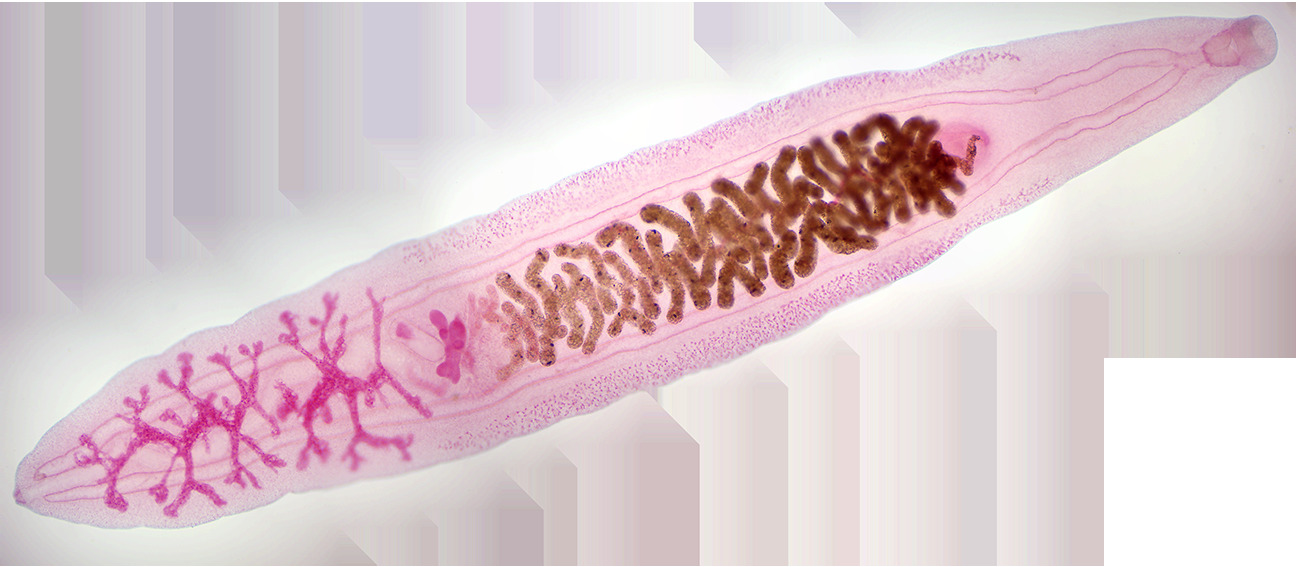
\includegraphics[width=0.7\linewidth]{./figures/rotifera/clonorchis_sinensis_wm}

}

\caption{\emph{Clonorchis sinensis}.}\label{fig:clonorchis}
\end{figure}

\begin{figure}

{\centering 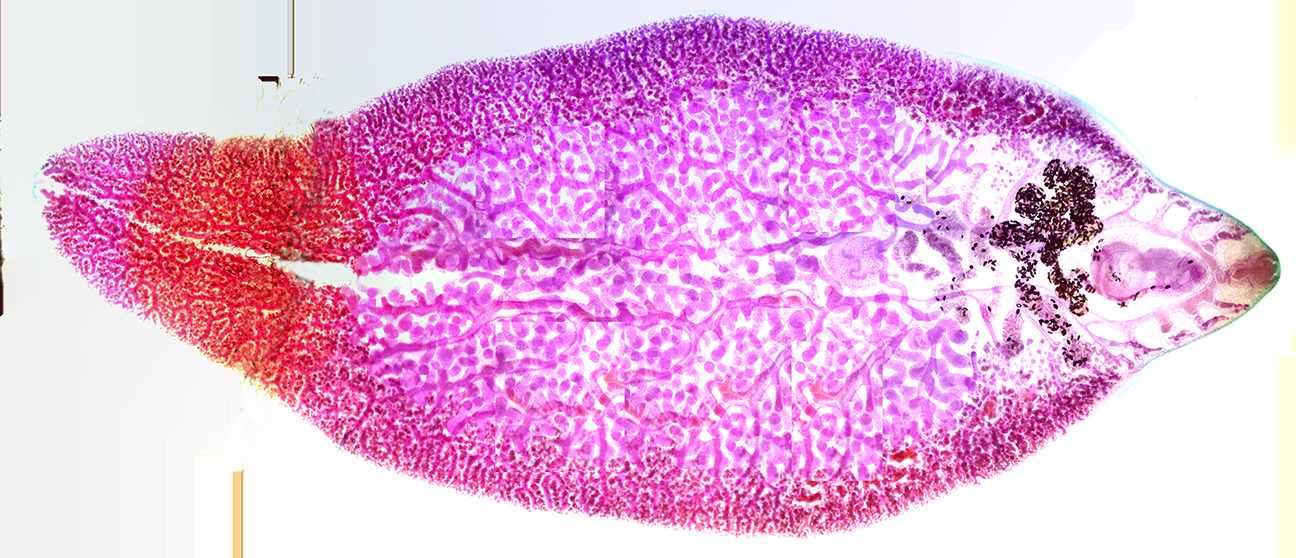
\includegraphics[width=0.7\linewidth]{./figures/rotifera/fasciola_hepatica}

}

\caption{\emph{Fasciola hepatica}.}\label{fig:fasciola}
\end{figure}

\section{\texorpdfstring{
\emph{Schistosoma}}{Schistosoma}}\label{Schistosoma}


\href{https://en.wikipedia.org/wiki/Schistosoma_mansoni}{\emph{Schistosoma
mansoni}} is a water-borne parasite of humans, and belongs to the group
of blood flukes (\emph{Schistosoma}). The adult lives in the blood vessels
(mesenteric veins) near the human intestine. It causes intestinal
schistosomiasis. Clinical symptoms are caused by the eggs. As the
leading cause of schistosomiasis in the world, it is one of the most prevalent
parasite in humans. It is classified as a neglected tropical disease. As
of 2016, 206.5 million people have schistosomiasis and \emph{S. mansoni} is the
major parasite. It is found in Africa, the Middle East, the Caribbean,
Brazil, Venezuela and Suriname.

Unlike other flukes (trematodes) in which sexes are not separate
(monoecious), schistosomes are unique in that adults are divided into
males and females, thus, (dioecious). However, the two adults live in
permanent partnership, a condition called in copula; for this, they are
considered as hermaphrodites. The life cycle of schistosomes includes
two hosts: humans as definitive hosts, where the parasite undergoes
sexual reproduction, and snails as intermediate hosts, where a series of
asexual reproductive takes place. \emph{S. mansoni} is transmitted through
water, where freshwater snails of the genus \emph{Biomphalaria} act as
intermediate hosts. The larvae are able to live in water and infect the
hosts by directly penetrating the skin. Prevention of infection is done
by improved sanitation and killing the snails. Infection is treated with
praziquantel. S. mansoni was first noted by Theodor Maximillian Bilharz
in Egypt in 1851, while discovering \emph{S. haematobium}. Sir Patrick Manson
identified it as unique species in 1902.

After the eggs of the human-dwelling parasite are emitted in the faeces
and into the water, the ripe miracidium hatches out of the egg. The
hatching happens in response to temperature, light and dilution of
faeces with water. The miracidium searches for a suitable freshwater
snail belonging to the genus \emph{Biomphalaria}. Miracidia directly penetrate
the soft tissue of snail. Inside the snail, they lose their cilia and
develop into mother sporocysts. The sporocysts rapidly multiply by
asexual reproduction, each forming numerous daughter sporocysts. The
daughter sporocysts move to the liver and gonads of the snail, where
they undergo further growth. Within 2--4 weeks, they undergo
metamorphosis and give rise to fork-tailed cercariae. Stimulated by
light, hundreds of cercariae penetrate out of the snail into water.

The cercaria emerge from the snail during daylight and they propel
themselves in water with the aid of their bifurcated tail, actively
seeking out their final host. In water, they can live for up to 12
hours, and their maximum infectivity is between 1 and 9 hours after
emergence. When they recognise human skin, they penetrate it within a
very short time. This occurs in three stages, an initial attachment to
the skin, followed by the creeping over the skin searching for a
suitable penetration site, often a hair follicle, and finally
penetration of the skin into the epidermis using cytolytic secretions
from the cercarial post-acetabular, then pre-acetabular glands. On
penetration, the head of the cercaria transforms into an endoparasitic
larva, the schistosomule. Each schistosomule spends a few days in the
skin and then enters the circulation starting at the dermal lymphatics
and venules. Here, they feed on blood, regurgitating the haem as
hemozoin. The schistosomule migrates to the lungs (5--7 days
post-penetration) and then moves via circulation through the left side
of the heart to the hepatoportal circulation (\textgreater{}15 days)
where, if it meets a partner of the opposite sex, it develops into a
sexually mature adult and the pair migrate to the mesenteric veins. Such
pairings are monogamous.

Male schistosomes undergo normal maturation and morphological
development in the presence or absence of a female, although
behavioural, physiological and antigenic differences between males from
single-sex, as opposed to bisex, infections have been reported. On the
other hand, female schistosomes do not mature without a male. Female
schistosomes from single-sex infections are underdeveloped and exhibit
an immature reproductive system. Although the maturation of the female
worm seems to be dependent on the presence of the mature male, the
stimuli for female growth and for reproductive development seem to be
independent from each other.

The adult female worm resides within the adult male worm's gynaecophoric
canal, which is a modification of the ventral surface of the male,
forming a groove. The paired worms move against the flow of blood to
their final niche in the mesenteric circulation, where they begin egg
production (\textgreater{}32 days). The \emph{S. mansoni} parasites are found
predominantly in the small inferior mesenteric blood vessels surrounding
the large intestine and caecal region of the host. Each female lays
approximately 300 eggs a day (one egg every 4.8 minutes), which are
deposited on the endothelial lining of the venous capillary walls. Most
of the body mass of female schistosomes is devoted to the reproductive
system. The female converts the equivalent of almost her own body dry
weight into eggs each day. The eggs move into the lumen of the host's
intestines and are released into the environment with the faeces.

\section{\texorpdfstring{View Prepared Slides of
\emph{Schistosoma}}{View Prepared Slides of Schistosoma}}\label{view-prepared-slides-of-schistosoma}

\begin{enumerate}
\def\labelenumi{\arabic{enumi}.}
\tightlist
\item
  Cercariae w.m. (Figure \ref{fig:cercaria}).
\end{enumerate}

\begin{figure}

{\centering 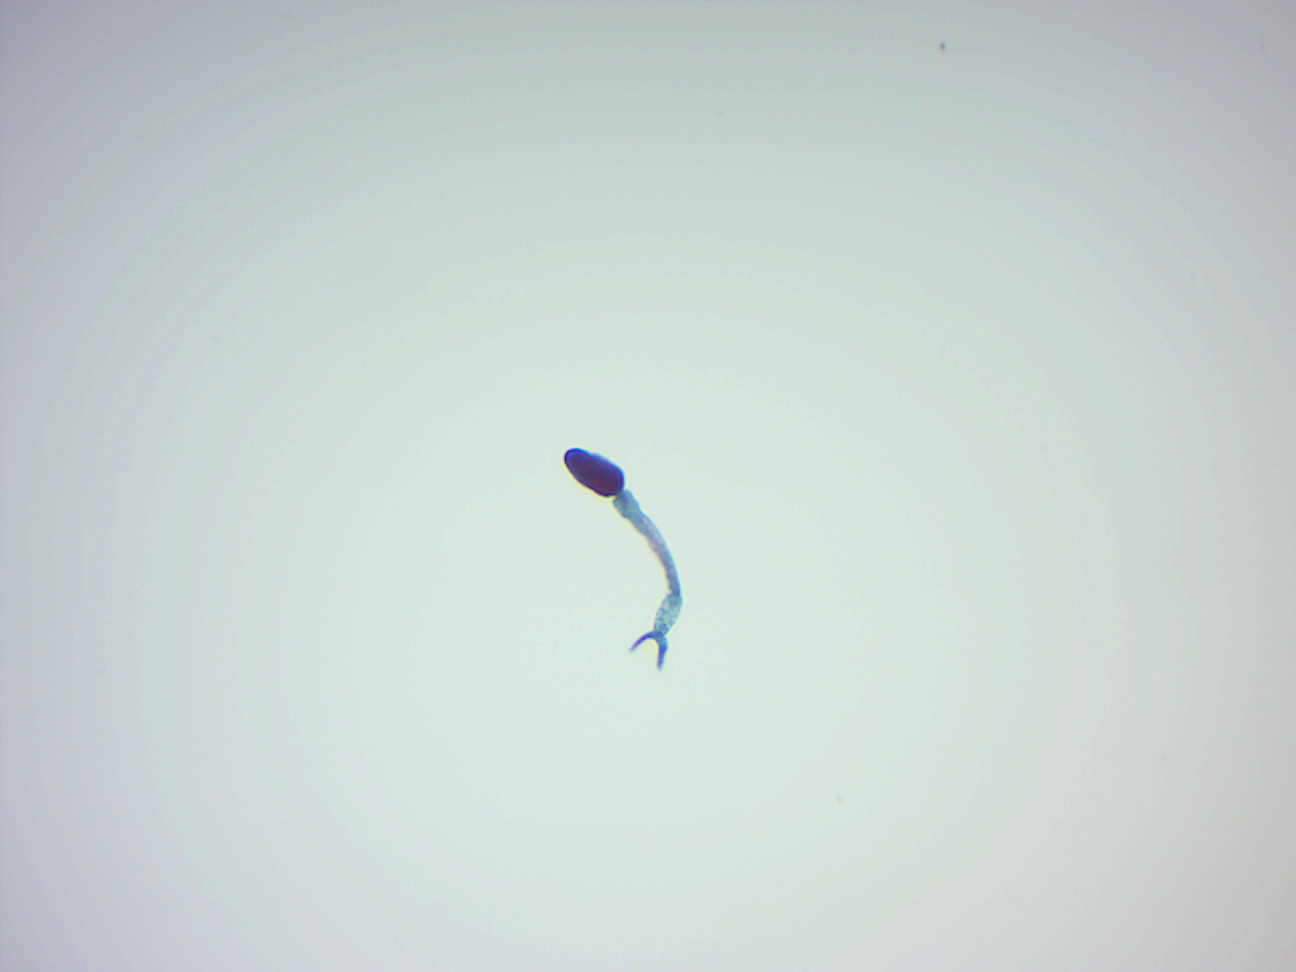
\includegraphics[width=0.7\linewidth]{./figures/rotifera/cercaria}

}

\caption{\emph{Schistosoma cercaria}.}\label{fig:cercaria}
\end{figure}

\section{Monogenea}\label{monogenea}

Monogeneans are a group of ectoparasite which are commonly found on the
skin, gills, or fins of fish. They have a direct life cycle and do not
require an intermediate host. Adults are hermaphrodites, meaning they
have both male and female reproductive structures.

\section{Molluska}\label{molluska}

\href{https://en.wikipedia.org/wiki/Mollusca}{Molluska} are a large
phylum of invertebrate animals whose members are known as mollusks.
Around 85,000 extant species of mollusks are recognized. Mollusks are
the largest marine phylum, comprising about 23\% of all the named marine
organisms. Numerous mollusks also live in freshwater and terrestrial
habitats. They are highly diverse, not just in size and in anatomical
structure, but also in behavior and in habitat. The phylum is typically
divided into 9 or 10 taxonomic classes, of which two are entirely
extinct. Cephalopod mollusks, such as squid, cuttlefish and octopus, are
among the most neurologically advanced of all invertebrates---and either
the giant squid or the colossal squid is the largest known invertebrate
species. The gastropods (snails and slugs) are by far the most numerous
mollusks in terms of classified species, and account for 80\% of the
total.

The three most universal features defining modern mollusks are a mantle
with a significant cavity used for breathing and excretion, the presence
of a radula (except for bivalves), and the structure of the nervous
system. Other than these things, mollusks express great morphological
diversity, so many textbooks base their descriptions on a ``hypothetical
ancestral mollusk'' (see image below). This has a single,
``limpet-like'' shell on top, which is made of proteins and chitin
reinforced with calcium carbonate, and is secreted by a mantle covering
the whole upper surface. The underside of the animal consists of a
single muscular ``foot''. Although mollusks are coelomates, the coelom
tends to be small. The main body cavity is a hemocoel through which
blood circulates; their circulatory systems are mainly open. The
``generalized'' mollusk's feeding system consists of a rasping
``tongue'', the radula, and a complex digestive system in which exuded
mucus and microscopic, muscle-powered ``hairs'' called cilia play
various important roles. The generalized mollusk has two paired nerve
cords, or three in bivalves. The brain, in species that have one,
encircles the esophagus. Most mollusks have eyes, and all have sensors
to detect chemicals, vibrations, and touch. The simplest type of
molluskan reproductive system relies on external fertilization, but more
complex variations occur. All produce eggs, from which may emerge
trochophore larvae, more complex veliger larvae, or miniature adults.

Good evidence exists for the appearance of gastropods, cephalopods and
bivalves in the Cambrian period 541 to 485.4 million years ago.

Mollusks have been and still are an important food source for
anatomically modern humans. However there is a risk of food poisoning
from toxins which can accumulate in certain mollusks under specific
conditions, and because of this, many countries have regulations to
reduce this risk. Mollusks have, for centuries, also been the source of
important luxury goods, notably pearls, mother of pearl, Tyrian purple
dye, and sea silk. Their shells have also been used as money in some
preindustrial societies.

Mollusk species can also represent hazards or pests for human
activities. Schistosomiasis (also known as bilharzia, bilharziosis or
snail fever) is transmitted to humans via water snail hosts, and affects
about 200 million people. Snails and slugs can also be serious
agricultural pests, and accidental or deliberate introduction of some
snail species into new environments has seriously damaged some
ecosystems.

\section{Bivalvia}\label{bivalvia}

\href{https://en.wikipedia.org/wiki/Bivalvia}{Bivalves} are a class of
marine and freshwater mollusks that have laterally compressed bodies
enclosed by a shell consisting of two hinged parts. Bivalves as a group
have no head and they lack some usual molluskan organs like the radula
and the odontophore (the cartilage which underlies and supports the
radula and forms a ribbon of ``teeth''). They include the clams,
oysters, cockles, mussels, scallops, and numerous other families that
live in saltwater, as well as a number of families that live in
freshwater. The majority are filter feeders. The gills evolved into a
specialized respiratory organ for feeding and breathing called
ctenidium. Most bivalves bury themselves in sediment where they are
relatively safe from predation. Others lie on the sea floor or attach
themselves to rocks or other hard surfaces. Some bivalves, such as the
scallops and file shells, can swim. The shipworms bore into wood, clay,
or stone and live inside these substances.

The shell of a bivalve is composed of calcium carbonate, and consists of
two, usually similar, parts called valves. These are joined together
along one edge (the hinge line) by a flexible ligament that, usually in
conjunction with interlocking ``teeth'' on each of the valves, forms the
hinge. This arrangement allows the shell to be opened and closed without
the two halves detaching. The shell is typically bilaterally
symmetrical, with the hinge lying in the sagittal plane. Adult shell
sizes of bivalves vary from fractions of a millimeter to over a meter in
length, but the majority of species do not exceed 10 cm.

Bivalves appear in the fossil record first in the early Cambrian more
than 500 million years ago. The total number of living species is about
9,200.

The sexes are usually separate in bivalves but some hermaphroditism is
known. The gonads are located close to the intestines, and either open
into the nephridia, or through a separate pore into the mantle cavity.
The ripe gonads of male and females release sperm and eggs into the
water column. Spawning may take place continually or be triggered by
environmental factors such as day length, water temperature, or the
presence of sperm in the water.

Fertilization is usually external. Typically, a short stage lasts a few
hours or days before the eggs hatch into trochophore larvae. These later
develop into veliger larvae which settle on the seabed and undergo
metamorphosis into juveniles. In some species, such as those in the
genus Lasaea, females draw water containing sperm in through their
inhalant siphons and fertilization takes place inside the female. These
species then brood the young inside their mantle cavity, eventually
releasing them into the water column as veliger larvae or as crawl-away
juveniles.

Most of the bivalve larvae that hatch from eggs in the water column feed
on diatoms or other phytoplankton. In temperate regions, about 25\% of
species are lecithotrophic, depending on nutrients stored in the yolk of
the egg where the main energy source is lipids. The larvae hatching out
of these rely on the energy reserves and do not feed.

\section{Clams}\label{clams}

\href{https://en.wikipedia.org/wiki/Clam}{Clams} have two shells of
equal size connected by two adductor muscles and have a powerful
burrowing foot. Some clams have life cycles of only one year, while at
least one may be over 500 years old. All clams have two calcareous
shells or valves joined near a hinge with a flexible ligament, and all
are filter feeders. A clam's shell consists of two (usually equal)
valves, which are connected by a hinge joint and a ligament that can be
external or internal. The ligament provides tension to bring the valves
apart, while one or two adductor muscles can contract to close the
valves. Clams also have kidneys, a heart, a mouth, a stomach, a nervous
system and an anus. Many have a siphon.

Clams are
\href{https://en.wikipedia.org/wiki/Sequential_hermaphroditism}{protandrous
hermaphrodites} which means that they begin life as males but by the end
of the first year approximately half of the population will change to
females. Male clams release sperm into the water which stimulates
females to expel eggs. A female may spawn several times each year,
producing millions of eggs. Within 12 to 14 hours, the fertilized egg
hatches into a microscopic creature called a trochophore larva (from the
ancient Greek trókhos, meaning ``wheel'', and phoréō, meaning ``to bear,
to carry'' because the larva is bearing a wheel-shaped band of cilia).
In less than a day, it transforms into a veliger larva (from Latin velum
``sail, curtain, covering, veil'' and -ger ``bearing''), a free-swimming
animal that has tiny wing-like lobes that propel it through the water.
The foot, shell and body organs begin to form during the veliger stage,
which lasts approximately 6 to 10 days. As the tiny shell develops, the
veliger drops to the sea floor and sheds its lobes. When it touches
bottom, it sends out thin filaments to hold it in place. As the clam
matures, a muscular foot will replace these filaments, allowing the clam
to bury itself in the sediments with only its siphons protruding.

\section{Gastropoda}\label{gastropoda}

\href{https://en.wikipedia.org/wiki/Gastropoda}{Gastropods} (previously
known as univalves) are a major part of the phylum Molluska, and are the
most highly diversified class in the phylum, with 65,000 to 80,000
living snail and slug species.

In the older classification of the gastropods, there were four
subclasses:

\begin{enumerate}
\def\labelenumi{\arabic{enumi}.}
\tightlist
\item
  Opisthobranchia (gills to the right and behind the heart).
\item
  Gymnomorpha (no shell)
\item
  Prosobranchia (gills in front of the heart).
\item
  Pulmonata (with a lung instead of gills)
\end{enumerate}

The class Gastropoda has an extraordinary diversification of habitats.
Representatives live in gardens, woodland, deserts, and on mountains; in
small ditches, great rivers and lakes; in estuaries, mudflats, the rocky
intertidal, the sandy subtidal, in the abyssal depths of the oceans
including the hydrothermal vents, and numerous other ecological niches,
including parasitic ones.

Although the name ``snail'' can be, and often is, applied to all the
members of this class, commonly this word means only those species with
an external shell big enough that the soft parts can withdraw completely
into it. Those gastropods without a shell, and those with only a very
reduced or internal shell, are usually known as slugs; those with a
shell into which they cannot withdraw are termed limpets.

The marine shelled species of gastropod include species such as abalone,
conches, periwinkles, whelks, and numerous other sea snails that produce
seashells that are coiled in the adult stage---though in some, the
coiling may not be very visible, for example in cowries. In a number of
families of species, such as all the various limpets, the shell is
coiled only in the larval stage, and is a simple conical structure after
that

Gastropods typically have a well-defined head with two or four sensory
tentacles with eyes, and a ventral foot, which gives them their name
(Greek gaster, stomach, and poda, feet). The upper pair of tentacles on
the head of \emph{Helix pomatia} have eye spots, but the main sensory organs of
the snail are sensory receptors for olfaction, situated in the
epithelium of the tentacles.

Sensory organs of gastropods include olfactory organs, eyes, statocysts
and mechanoreceptors. Gastropods have no hearing. In terrestrial
gastropods (land snails and slugs), the olfactory organs, located on the
tips of the four tentacles, are the most important sensory organ. The
majority of gastropods have simple visual organs, eye spots either at
the tip or base of the tentacles. However, ``eyes'' in gastropods range
from simple ocelli that only distinguish light and dark, to more complex
pit eyes, and even to lens eyes. In land snails and slugs, vision is not
the most important sense, because they are mainly nocturnal animals. The
nervous system of gastropods includes the peripheral nervous system and
the central nervous system. The central nervous system consists of
ganglia connected by nerve cells.

The radula of a gastropod is usually adapted to the food that a species
eats. The simplest gastropods are the limpets and abalones, herbivores
that use their hard radula to rasp at seaweeds on rocks. Many marine
gastropods are burrowers, and have a siphon that extends out from the
mantle edge. Sometimes the shell has a siphonal canal to accommodate
this structure. A siphon enables the animal to draw water into their
mantle cavity and over the gill. They use the siphon primarily to
``taste'' the water to detect prey from a distance. Gastropods with
siphons tend to be either predators or scavengers.

Almost all marine gastropods breathe with a gill, but many freshwater
species, and the majority of terrestrial species, have a pallial lung.

Gastropods have open circulatory system and the transport fluid is
hemolymph. Hemocyanin is present in the hemolymph as the respiratory
pigment.

The primary organs of excretion in gastropods are nephridia, which
produce either ammonia or uric acid as a waste product. The nephridium
also plays an important role in maintaining water balance in freshwater
and terrestrial species. Additional organs of excretion, at least in
some species, include pericardial glands in the body cavity, and
digestive glands opening into the stomach. In many marine gastropods
other than the opisthobranchs, there are separate sexes; most land
gastropods, however, are hermaphrodites.

\section{View Prepared Slides of
Molluska}\label{view-prepared-slides-of-molluska}

\begin{enumerate}
\def\labelenumi{\arabic{enumi}.}
\tightlist
\item
  Snail Radula w.m. (Figure \ref{fig:radula})

  \begin{itemize}
  \tightlist
  \item
    Locate rows of chitinous teeth.
  \end{itemize}
\end{enumerate}

\begin{figure}

{\centering 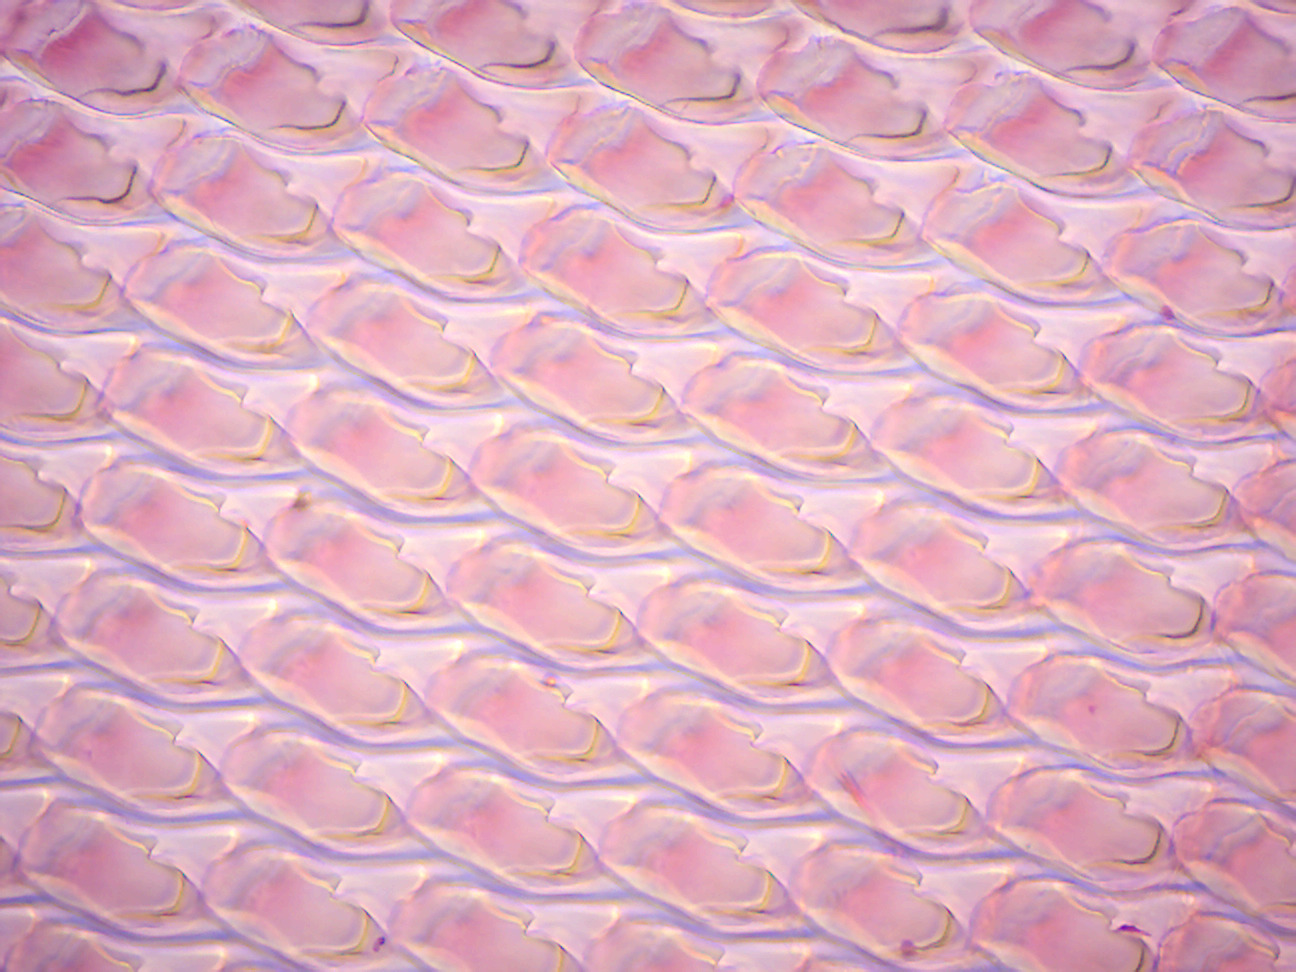
\includegraphics[width=0.7\linewidth]{./figures/rotifera/snail_radula}

}

\caption{Snail radula.}\label{fig:radula}
\end{figure}

\section{Cephalopoda}\label{cephalopoda}

\href{https://en.wikipedia.org/wiki/Cephalopod}{Cephalopods} are members
of the molluskan class Cephalopoda (Greek plural kephalópoda;
``head-feet'') such as a squid, octopus or nautilus. These exclusively
marine animals are characterized by bilateral body symmetry, a prominent
head, and a set of arms or tentacles modified from the primitive
molluskan foot. About 800 living species of cephalopods have been
identified. Two important extinct taxa are the Ammonoidea (ammonites)
and Belemnoidea (belemnites).

Cephalopods are found in all the oceans of Earth. Cephalopods occupy
most of the depth of the ocean, from the abyssal plain to the sea
surface.

Cephalopods are widely regarded as the most intelligent of the
invertebrates, and have well developed senses and large brains (larger
than those of gastropods). The nervous system of cephalopods is the most
complex of the invertebrates.

The brain is protected in a cartilaginous cranium. The giant nerve
fibers of the cephalopod mantle have been widely used for many years as
experimental material in neurophysiology; their large diameter (due to
lack of myelination) makes them relatively easy to study compared with
other animals. Many cephalopods are social creatures.

Cephalopods have advanced vision, can detect gravity with statocysts,
and have a variety of chemical sense organs. Octopuses use their arms to
explore their environment and can use them for depth perception.

Most cephalopods rely on vision to detect predators and prey, and to
communicate with one another. Consequently, cephalopod vision is acute:
training experiments have shown that the common octopus can distinguish
the brightness, size, shape, and horizontal or vertical orientation of
objects. The morphological construction gives cephalopod eyes the same
performance as sharks'; however, their construction differs, as
cephalopods lack a cornea, and have an everted retina. Cephalopods' eyes
are also sensitive to the plane of polarization of light. Surprisingly,
given their ability to change color, all octopodes and most cephalopods
are considered to be color blind. Coleoid cephalopods (octopus, squid,
cuttlefish) have a single photoreceptor type and lack the ability to
determine color by comparing detected photon intensity across multiple
spectral channels. When camouflaging themselves, they use their
chromatophores to change brightness and pattern according to the
background they see, but their ability to match the specific color of a
background may come from cells such as iridophores and leucophores that
reflect light from the environment. They also produce visual pigments
throughout their body, and may sense light levels directly from their
body.

Cephalopods are the only mollusks with a closed circulatory system. Like
most mollusks, cephalopods use hemocyanin, a copper-containing protein,
rather than hemoglobin, to transport oxygen. As a result, their blood is
colorless when deoxygenated and turns blue when exposed to air.

Cephalopods exchange gases with the seawater by forcing water through
their gills, which are attached to the roof of the organism. Water
enters the mantle cavity on the outside of the gills, and the entrance
of the mantle cavity closes. When the mantle contracts, water is forced
through the gills, which lie between the mantle cavity and the funnel.
The water's expulsion through the funnel can be used to power jet
propulsion. The gills, which are much more efficient than those of other
mollusks, are attached to the ventral surface of the mantle cavity.

All living cephalopods have a two-part beak; most have a radula,
although it is reduced in most octopus. They feed by capturing prey with
their tentacles, drawing it into their mouth and taking bites from it.
They have a mixture of toxic digestive juices, some of which are
manufactured by symbiotic algae, which they eject from their salivary
glands onto their captured prey held in their mouth. These juices
separate the flesh of their prey from the bone or shell. The salivary
gland has a small tooth at its end which can be poked into an organism
to digest it from within.

The digestive gland itself is rather short. It has four elements, with
food passing through the crop, stomach and caecum before entering the
intestine. Most digestion, as well as the absorption of nutrients,
occurs in the digestive gland, sometimes called the liver. Nutrients and
waste materials are exchanged between the gut and the digestive gland
through a pair of connections linking the gland to the junction of the
stomach and caecum. Cells in the digestive gland directly release
pigmented excretory chemicals into the lumen of the gut, which are then
bound with mucus passed through the anus as long dark strings, ejected
with the aid of exhaled water from the funnel.

Most cephalopods possess a single pair of large nephridia. Filtered
nitrogenous waste is produced in the pericardial cavity of the branchial
hearts, each of which is connected to a nephridium by a narrow canal.
The canal delivers the excreta to a bladder-like renal sac, and also
resorbs excess water from the filtrate. Several outgrowths of the
lateral vena cava project into the renal sac, continuously inflating and
deflating as the branchial hearts beat. This action helps to pump the
secreted waste into the sacs, to be released into the mantle cavity
through a pore.

\section{Annelida}\label{annelida}

The \href{https://en.wikipedia.org/wiki/Annelid}{annelids} (Annelida,
from Latin anellus, ``little ring''), also known as the ringed worms or
segmented worms, are a large phylum, with over 17,000 extant species
including ragworms, earthworms, and leeches. The species exist in and
have adapted to various ecologies -- some in marine environments as
distinct as tidal zones and hydrothermal vents, others in fresh water,
and yet others in moist terrestrial environments.

The annelids are bilaterally symmetrical, triploblastic, coelomate,
invertebrate organisms. They also have parapodia for locomotion. Most
textbooks still use the traditional division into polychaetes (almost
all marine), oligochaetes (which include earthworms) and leech-like
species. Cladistic research since 1997 has radically changed this
scheme, viewing leeches as a sub-group of oligochaetes and oligochaetes
as a sub-group of polychaetes. In addition, the Pogonophora, Echiura and
Sipuncula, previously regarded as separate phyla, are now regarded as
sub-groups of polychaetes. Annelids are considered members of the
Lophotrochozoa, a ``super-phylum'' of protostomes that also includes
mollusks', \href{https://en.wikipedia.org/wiki/Brachiopod}{brachiopods},
flatworms and \href{https://en.wikipedia.org/wiki/Nemertea}{nemertea}.

The basic annelid form consists of multiple segments. Each segment has
the same sets of organs and, in most polychaetes, has a pair of
parapodia that many species use for locomotion. Septa separate the
segments of many species, but are poorly defined or absent in others,
and Echiura and Sipuncula show no obvious signs of segmentation. In
species with well-developed septa, the blood circulates entirely within
blood vessels, and the vessels in segments near the front ends of these
species are often built up with muscles that act as hearts. The septa of
such species also enable them to change the shapes of individual
segments, which facilitates movement by peristalsis (``ripples'' that
pass along the body) or by undulations that improve the effectiveness of
the parapodia. In species with incomplete septa or none, the blood
circulates through the main body cavity without any kind of pump, and
there is a wide range of locomotory techniques -- some burrowing species
turn their pharynges inside out to drag themselves through the sediment.

Although many species can reproduce asexually and use similar mechanisms
to regenerate after severe injuries, sexual reproduction is the normal
method in species whose reproduction has been studied. The minority of
living polychaetes whose reproduction and lifecycles are known produce
trochophore larvae, that live as plankton and then sink and metamorphose
into miniature adults. Oligochaetes are full hermaphrodites and produce
a ring-like cocoon around their bodies, in which the eggs and hatchlings
are nourished until they are ready to emerge.

Earthworms are Oligochaetes that support terrestrial food chains both as
prey and in some regions, are important in aeration and enriching of
soil. The burrowing of marine polychaetes, which may constitute up to a
third of all species in near-shore environments, encourages the
development of ecosystems by enabling water and oxygen to penetrate the
sea floor. In addition to improving soil fertility, annelids serve
humans as food and as bait. Scientists observe annelids to monitor the
quality of marine and fresh water. Although blood-letting is no longer
in favor with doctors, some leech species are regarded as endangered
species because they have been over-harvested for this purpose in the
last few centuries.

Since annelids are soft-bodied, their fossils are rare -- mostly jaws
and the mineralized tubes that some of the species secreted. Although
some late Ediacaran fossils may represent annelids, the oldest known
fossil that is identified with confidence comes from about 518 million
years ago in the early Cambrian period. Fossils of most modern mobile
polychaete groups appeared by the end of the Carboniferous, about 299
million years ago. Palaeontologists disagree about whether some body
fossils from the mid Ordovician, about 472 to 461 million years ago, are
the remains of oligochaetes, and the earliest indisputable fossils of
the group appear in the Tertiary period, which began 65 million years
ago.

\section{Earthworm}\label{earthworm}

An \href{https://en.wikipedia.org/wiki/Earthworm}{earthworm} is a
tube-shaped, segmented worm found in the phylum Annelida. Earthworms are
commonly found living in soil, feeding on live and dead organic matter.
An earthworm's digestive system runs through the length of its body. It
conducts respiration through its skin. It has a double transport system
composed of coelomic fluid that moves within the fluid-filled coelom and
a simple, closed blood circulatory system. It has a central and a
peripheral nervous system. The central nervous system consists of two
ganglia above the mouth, one on either side, connected to a nerve cord
running back along its length to motor neurons and sensory cells in each
segment. Large numbers of chemoreceptors are concentrated near its
mouth. Circumferential and longitudinal muscles on the periphery of each
segment enable the worm to move. Similar sets of muscles line the gut,
and their actions move the digesting food toward the worm's anus.

Earthworms are hermaphrodites--each individual carries both male and
female sex organs. They lack either an internal skeleton or exoskeleton,
but maintain their structure with fluid-filled coelom chambers that
function as a hydrostatic skeleton.

Depending on the species, an adult earthworm can be from 10 mm long and
1 mm wide to 3 m long and over 25 mm wide, but the typical
\href{https://en.wikipedia.org/wiki/Lumbricus_terrestris}{\emph{Lumbricus
terrestris}} grows to about 360 mm long. Probably the longest worm on
confirmed records is
\href{https://en.wikipedia.org/wiki/Amynthas_mekongianus}{\emph{Amynthas
mekongianus}} that extends up to 3 m in the mud along the banks of the
Mekong River in Southeast Asia.

From front to back, the basic shape of the earthworm is a cylindrical
tube, divided into a series of segments (called metamerisms) that
compartmentalize the body. Furrows are generally externally visible on
the body demarking the segments; dorsal pores and nephridiopores exude a
fluid that moistens and protects the worm's surface, allowing it to
breathe. Except for the mouth and anal segments, each segment carries
bristle-like hairs called lateral setae used to anchor parts of the body
during movement; species may have four pairs of setae on each segment or
more than eight sometimes forming a complete circle of setae per
segment.

Generally, within a species, the number of segments found is consistent
across specimens, and individuals are born with the number of segments
they will have throughout their lives. The first body segment (segment
number 1) features both the earthworm's mouth and, overhanging the
mouth, a fleshy lobe called the prostomium, which seals the entrance
when the worm is at rest, but is also used to feel and chemically sense
the worm's surroundings. Some species of earthworm can even use the
prehensile prostomium to grab and drag items such as grasses and leaves
into their burrow.

An adult earthworm develops a belt-like glandular swelling, called the
clitellum, which covers several segments toward the front part of the
animal. This is part of the reproductive system and produces egg
capsules. The posterior is most commonly cylindrical like the rest of
the body, but depending on the species, may also be quadrangular,
octagonal, trapezoidal, or flattened. The last segment is called the
periproct; the earthworm's anus, a short vertical slit, is found on this
segment.

The exterior of an individual segment is a thin cuticle over skin,
commonly pigmented red to brown, which has specialized cells that
secrete mucus over the cuticle to keep the body moist and ease movement
through soil. Under the skin is a layer of nerve tissue, and two layers
of muscles---a thin outer layer of circular muscle, and a much thicker
inner layer of longitudinal muscle. Interior to the muscle layer is a
fluid-filled chamber called a coelom that by its pressurization provides
structure to the worm's boneless body. The segments are separated from
each other by septa (the plural of ``septum'') which are perforated
transverse walls, allowing the coelomic fluid to pass between segments.
A pair of structures called nephrostomes are located at the back of each
septum; a nephric tubule leads from each nephrostome through the septum
and into the following segment. This tubule then leads to the main body
fluid filtering organ, the nephridium or metanephridium, which removes
metabolic waste from the coelomic fluid and expels it through pores
called nephridiopores on the worm's sides; usually two nephridia
(sometimes more) are found in most segments. At the center of a worm is
the digestive tract, which runs straight through from mouth to anus
without coiling, and is flanked above and below by blood vessels (the
dorsal blood vessel and the ventral blood vessel as well as a subneural
blood vessel) and the ventral nerve cord, and is surrounded in each
segment by a pair of pallial blood vessels that connect the dorsal to
the subneural blood vessels.

The earthworm's nervous system has three parts: the central nervous
system (CNS), peripheral nervous system and the sympathetic nervous
system.

The gut of the earthworm is a straight tube which extends from the
worm's mouth to its anus. It is differentiated into a buccal cavity
(generally running through the first one or two segments of the
earthworm), pharynx (running generally about four segments in length),
esophagus, crop, gizzard (usually) and intestine. Food enters in the
mouth. The pharynx acts as a suction pump; its muscular walls draw in
food. In the pharynx, the pharyngeal glands secrete mucus. Food moves
into the esophagus. From there the food passes into the crop and
gizzard. In the gizzard, strong muscular contractions grind the food
with the help of mineral particles ingested along with the food. Once
through the gizzard, food continues through the intestine for digestion.
Instead of being coiled like a mammalian intestine, an earthworm's
intestine increases surface area to increase nutrient absorption by
having many folds running along its length. The intestine has its own
pair of muscle layers like the body, but in reverse order---an inner
circular layer within an outer longitudinal layer.

The earthworm has a dual circulatory system in which both the coelomic
fluid and a closed circulatory system carry the food, waste, and
respiratory gases. The closed circulatory system has five main blood
vessels: the dorsal (top) vessel, which runs above the digestive tract;
the ventral (bottom) vessel, which runs below the digestive tract; the
subneural vessel, which runs below the ventral nerve cord; and two
lateroneural vessels on either side of the nerve cord. The dorsal vessel
moves the blood forward, while the other four longitudinal vessels carry
the blood rearward. In segments seven through eleven, a pair of aortic
arches rings the coelom and acts as hearts, pumping the blood to the
ventral vessel that acts as the aorta. The blood consists of ameboid
cells and hemoglobin dissolved in the plasma. The second circulatory
system derives from the cells of the digestive system that line the
coelom.

The excretory system contains a pair of nephridia in every segment,
except for the first three and the last ones. The waste in the coelom
fluid from a forward segment is drawn in by the beating of cilia of the
nephrostome. From there it is carried through the septum (wall) via a
tube which forms a series of loops entwined by blood capillaries that
also transfer waste into the tubule of the nephrostome. The excretory
wastes are then finally discharged through a pore on the worm's side.

Earthworms have no special respiratory organs. Gases are exchanged
through the moist skin and capillaries, where the oxygen is picked up by
the hemoglobin dissolved in the blood plasma and carbon dioxide is
released. Water, as well as salts, can also be moved through the skin by
active transport.

Mating occurs on the surface, most often at night. Earthworms are
hermaphrodites; that is, they have both male and female sexual organs.
The sexual organs are located in segments 9 to 15. Earthworms have one
or two pairs of testes contained within sacs. The two or four pairs of
seminal vesicles produce, store and release the sperm via the male
pores. Ovaries and oviducts in segment 13 release eggs via female pores
on segment 14, while sperm is expelled from segment 15. One or more
pairs of spermathecae are present in segments 9 and 10 (depending on the
species) which are internal sacs that receive and store sperm from the
other worm during copulation. As a result, segment 15 of one worm exudes
sperm into segments 9 and 10 with its storage vesicles of its mate. Some
species use external spermatophores for sperm transfer. Copulation and
reproduction are separate processes in earthworms. The mating pair
overlap front ends ventrally and each exchanges sperm with the other.
The clitellum becomes very reddish to pinkish in color. Sometime after
copulation, long after the worms have separated, the clitellum (behind
the spermathecae) secretes material which forms a ring around the worm.
The worm then backs out of the ring, and as it does so, it injects its
own eggs and the other worm's sperm into it. As the worm slips out of
the ring, the ends of the cocoon seal to form a vaguely lemon-shaped
incubator (cocoon) in which the embryonic worms develop. They emerge as
small, but fully formed earthworms, but lack their sex structures, which
develop in about 60 to 90 days. They attain full size in about one year.
Scientists predict that the average lifespan under field conditions is
four to eight years, while most garden varieties live only one to two
years.

\section{View Living Organisms}\label{view-living-organisms-3}

\begin{enumerate}
\def\labelenumi{\arabic{enumi}.}
\tightlist
\item
  Turbellaria
\item
  Rotifers
\end{enumerate}

\begin{figure}

{\centering 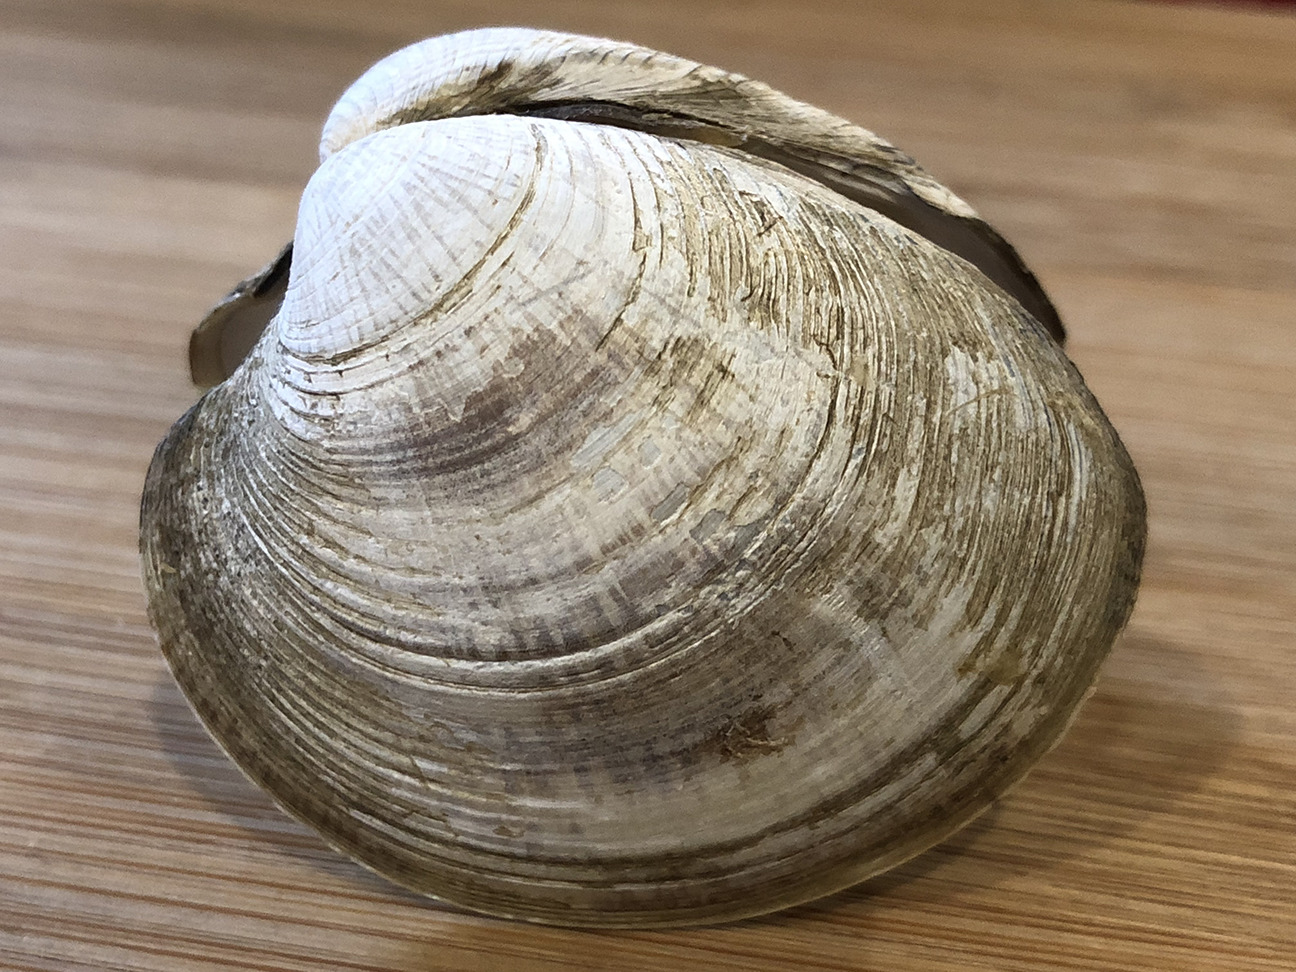
\includegraphics[width=0.7\linewidth]{./figures/rotifera/clam}

}

\caption{Clam}\label{fig:clam}
\end{figure}

\section{Clam Dissection}\label{clam-dissection}

\begin{enumerate}
\def\labelenumi{\arabic{enumi}.}
\tightlist
\item
  Get a dissecting pan, a scalpel, forceps, and a pointer.
\item
  Get a clam.
\item
  Identify the anterior and posterior ends of the clam as well as the
  dorsal, ventral, and left and right lateral surfaces (Figure
  \ref{fig:clam}).
\item
  Place a clam in a dissecting tray with the left side up facing you.
\item
  Locate the umbo, the bump at the anterior end of the valve. This is
  the oldest part of the clam shell. Find the hinge ligament which
  hinges the valves together and observe the growth rings.
\item
  Locate the adductor muscles. With your blade pointing toward the
  dorsal edge, slide your scalpel between the two valves \& and cut
  through the anterior adductor muscle, cutting as close to the shell as
  possible.
\item
  Repeat step 6 in cutting the posterior adductor muscle.
\item
  Bend the left valve back so it lies flat on the tray. Once both
  adductor muscles have been cut away from the left shell, the shell can
  be opened easily.
\item
  Locate the muscle ``scars'' on the inner surface of the left valve.
  The adductor muscles were attached here to hold the clam closed.
\item
  Identify the mantle, the tissue that lines both valves \& covers the
  soft body of the clam. Find the mantle cavity, the space inside the
  mantle.
\item
  Locate two openings on the posterior end of the clam. The more ventral
  opening is the incurrent siphon that carries water into the clam and
  the more dorsal opening is the excurrent siphon where wastes and water
  leave. The large muscle attached to the siphons is called the siphon
  retractor muscle. There would be another one on the right side. These
  muscles pull the siphon in. Most clams can retract the siphons
  completely into the shell.
\item
  Lift the mantle up. Notice how thin it is. Remove the mantle to expose
  the gills and the foot. Notice the structure of the gills. Bivalves
  are filter feeders. The gills are used to strain plankton out of the
  water, as well as to remove oxygen from the water. There are another
  pair of gills on the right side of the clam.
\item
  Observe the muscular foot of the clam, which is ventral to the gills.
  Note the hatchet shape of the foot used to burrow into mud or sand.
\item
  Locate the labial palps, flaplike structures that surround and guide
  food into the clam's mouth. The palps are anterior to the gills \&
  ventral to the anterior adductor muscle. Between the palps, find the
  mouth.
\item
  Carefully make an incision in the middle of the visceral mass to view
  the internal organs.
\item
  Locate the spongy, yellowish reproductive organs.
\item
  Ventral to the umbo, find the digestive gland, a greenish structure
  that surrounds the stomach.
\item
  Locate the long, coiled intestine extending from the stomach.
\item
  Follow the intestine through the clam. Find the area near the dorsal
  surface that the intestine passes through called the pericardial area.
  Find the clam's heart in this area.
\item
  Continue following the intestine toward the posterior end of the clam.
  The heart is contained in a thin-walled sac called the pericardium
  near the top of the clam above the visceral mass. The tube-like
  structure that runs through the pericardium is the intestine.
\end{enumerate}

\section{Cleaning up}\label{cleaning-up}

\begin{enumerate}
\def\labelenumi{\arabic{enumi}.}
\tightlist
\item
  Dispose of the remains of the clam in the red biohazard bins.
\item
  Clean the dissection tray and instruments.
\end{enumerate}

\section{Earthworm Dissection}\label{earthworm-dissection}

\begin{enumerate}
\def\labelenumi{\arabic{enumi}.}
\tightlist
\item
  Get a dissecting pan, a scalpel, forceps, and a pointer.
\item
  Get an earhtworm.
\item
  Position your preserved earthworm dorsal side up and pin it down
  through the first segment and then again further back behind the
  clitellum (Figure \ref{fig:earthworm}).
\item
  Cut a slit in the dorsal surface near the posterior pin and extend the
  cut forward to the first segment. Be careful not to cut too deep.
\item
  Starting at the first segment, cut the septa (thin membranes) that
  internally divide the segments, so the skin can be laid flat. Use
  additional pins to hold the integument open and expose the organs.
\item
  Continue to lay the skin back until you have uncovered a centimeter or
  so of the intestine.
\item
  Locate and identify the five pairs of aortic arches, or hearts. Then
  find the dorsal blood vessel. Look for smaller blood vessels that
  branch from the dorsal blood vessel.
\item
  Starting at the anterior end, locate the muscular pharynx (food
  ingestion). This is followed by a tube-like esophagus which terminates
  in a crop (the wider organ) which serves as a storage stomach.
  Posterior to the crop is the gizzard. Gently press on the crop and
  gizzard to test their firmness. While the crop is soft and thin, the
  gizzard is muscular (soil is ground up and churned within the
  gizzard). The gizzard is followed by a long intestine in which both
  digestion and absorption occur. Undigested material is voided through
  the anus.
\item
  To find organs of the nervous system, push aside the digestive and
  circulatory system organs. Locate the ventral nerve cord. Trace the
  nerve cord forward to the nerve collar, which circles the pharynx.
  Find one pair of ganglia under the pharynx and another pair of ganglia
  above the pharynx. The ganglia above the pharynx serve as the brain of
  the earthworm.
\item
  Locate the nephridia. There are two in every segment.
\item
  Locate and identify a pair of ovaries in segment 13.
\item
  Look for two pairs of tiny testes in segments 10 and 11. To find these
  organs, you will again have to push aside some parts already
  dissected.
\end{enumerate}

\section{Cleaning up}\label{cleaning-up-1}

\begin{enumerate}
\def\labelenumi{\arabic{enumi}.}
\tightlist
\item
  Dispose of the remains of the earthworm in the red biohazard bins.
\item
  Clean the dissection tray and instruments and return them to the place
  where you picked them up.
\item
  Clean table tops with red bottled sanitizer
\item
  Wash hands before leaving class.
\end{enumerate}

\begin{figure}

{\centering 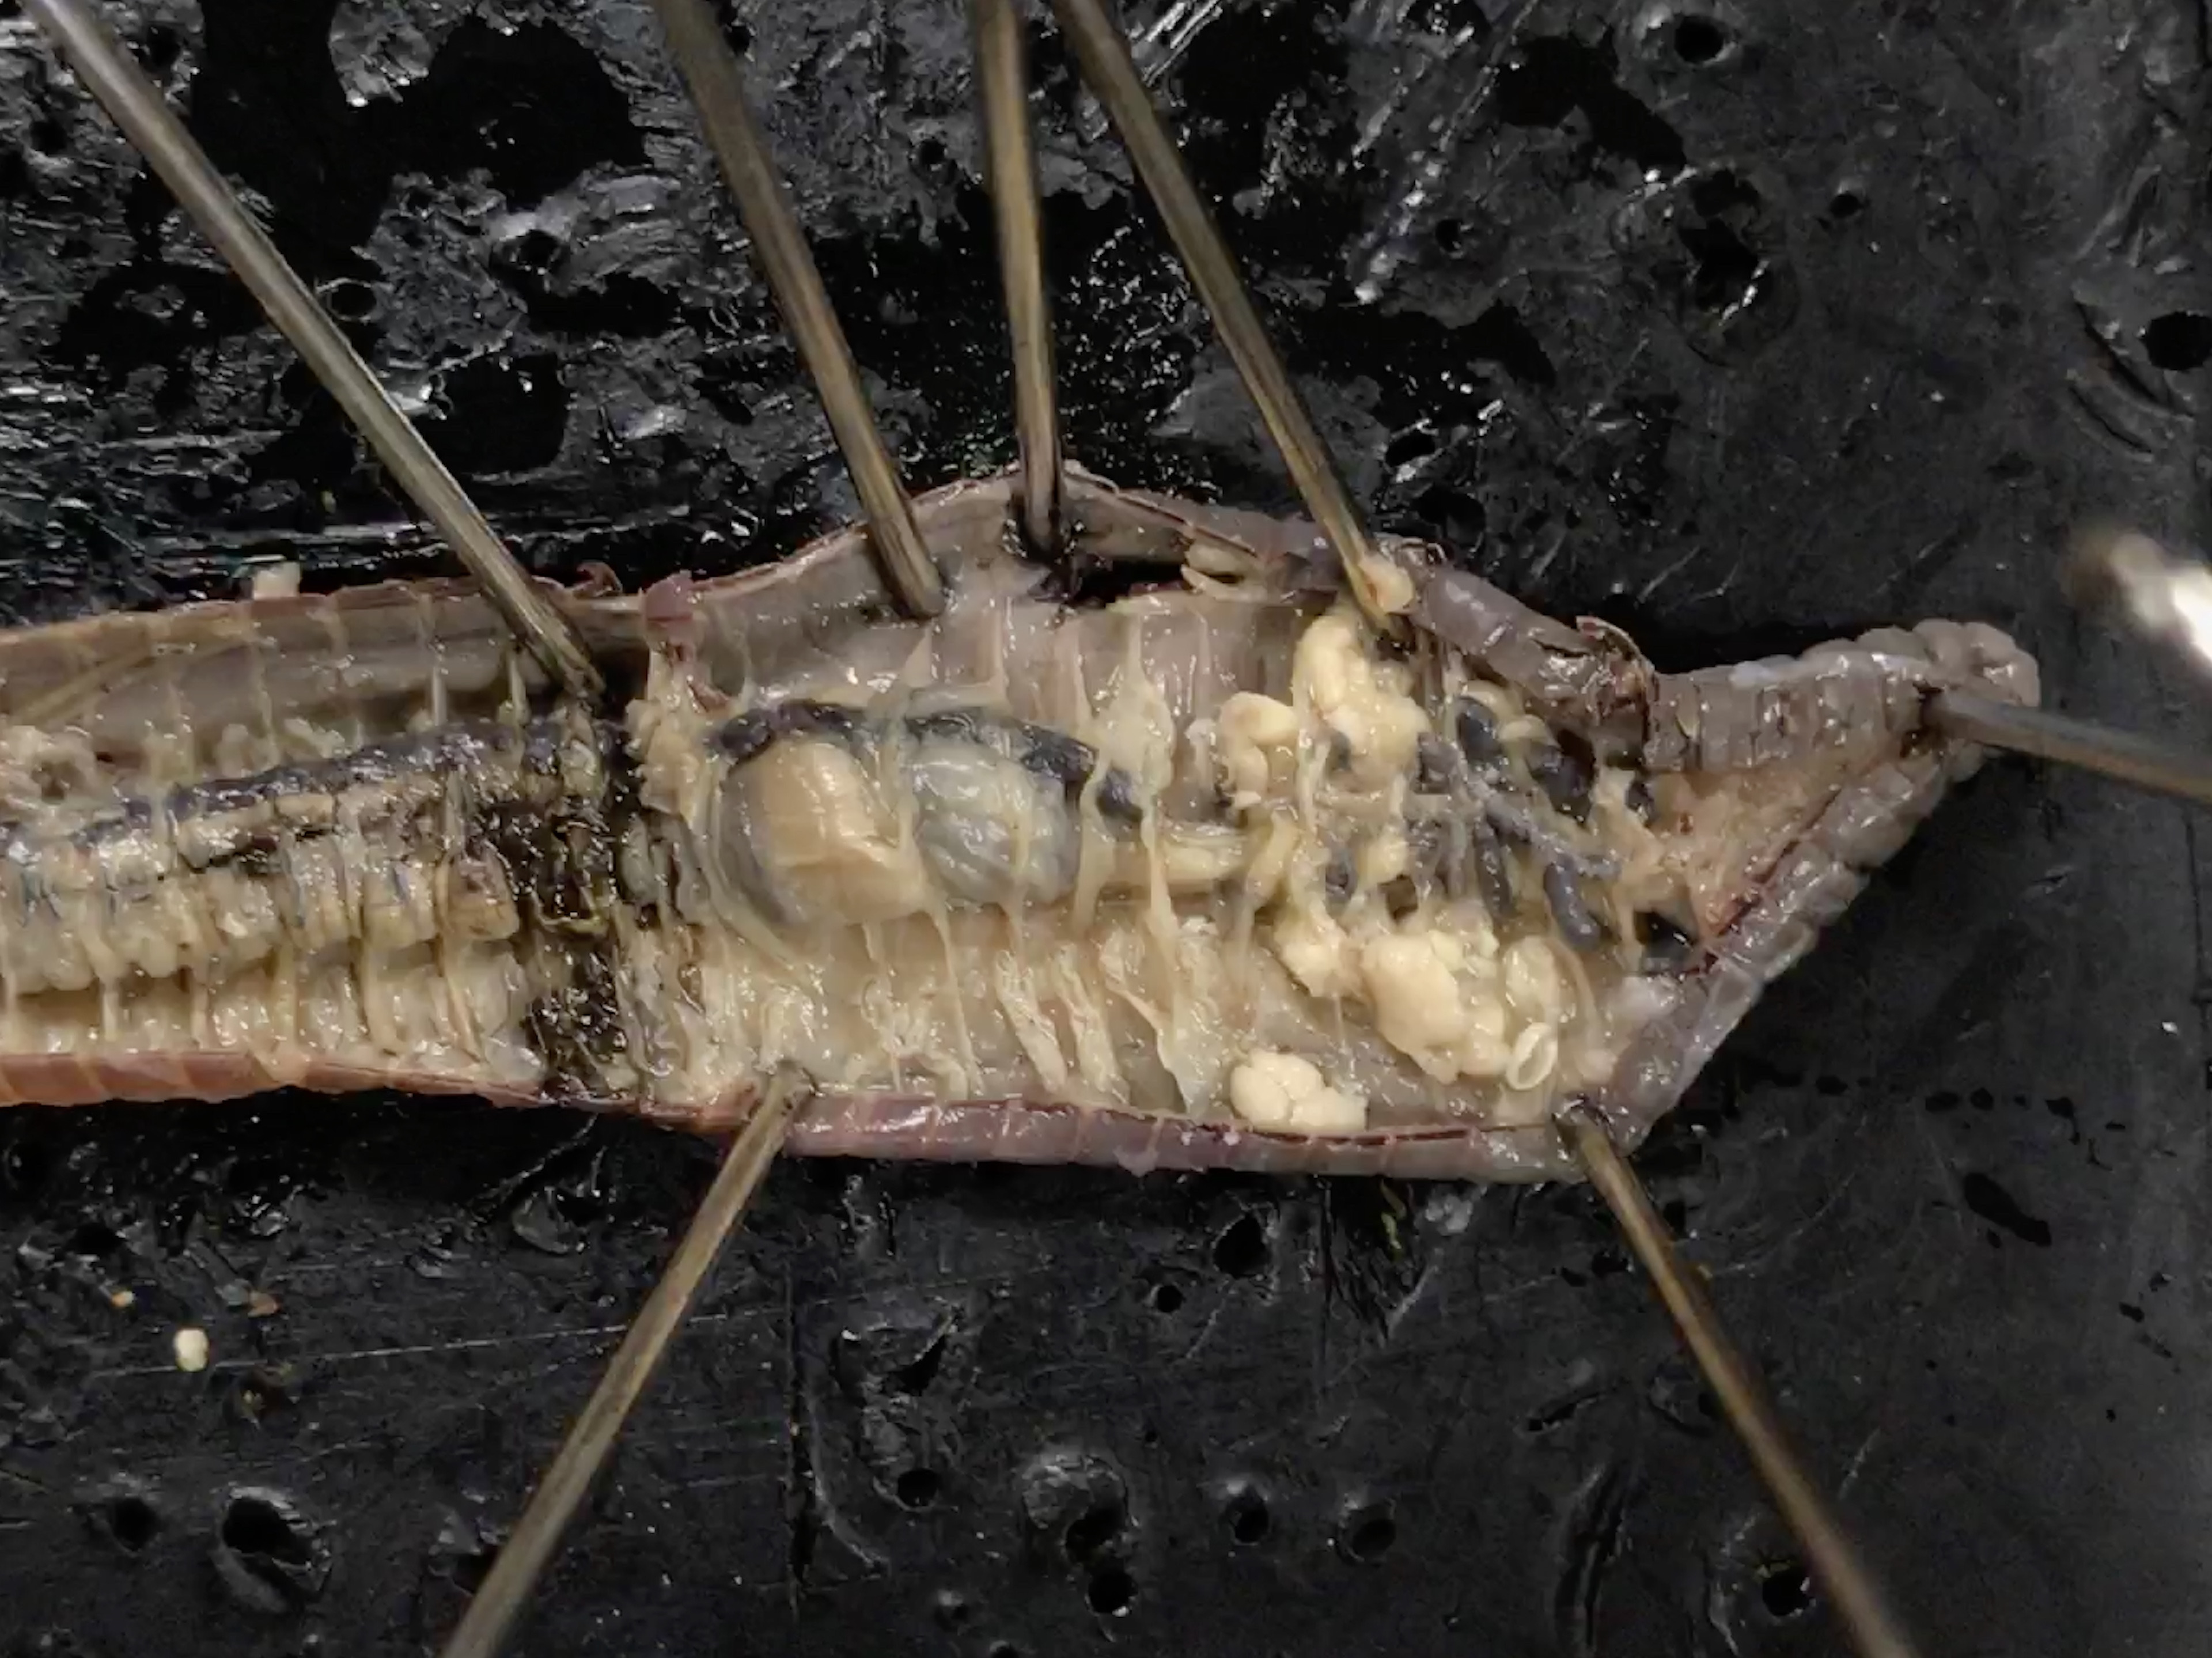
\includegraphics[width=0.7\linewidth]{./figures/rotifera/earthworm}

}

\caption{Earthworm dissection}\label{fig:earthworm}
\end{figure}

\section{Review Questions}\label{review-questions-4}

\begin{enumerate}
\def\labelenumi{\arabic{enumi}.}
\tightlist
\item
  What are rotifers?
\item
  What are flat worms?
\item
  What are mollusks?
\item
  What are annelids?
\item
  What is segmentation?
\item
  What is a radula?
\item
  What is a closed circulatory system?
\item
  What is an open circulatory system?
\end{enumerate}
